\chapter{MÓDULOS DE MEDICIÓN}
\label{Cap:Modulos}
Actualmente los SiPM juegan un importante rol en el campo de la física de altas energías \citep{Intro_SIPM_Sensl}, su estudio y caracterización toma cada vez más relevancia. Sin embargo, los equipos electrónicos para realizar dichos procedimientos son muy costosos y de difícil acceso, es por eso que en este proyecto se propone desarrollar un conjunto de módulos enfocados en la caracterización del voltaje de ruptura, la ganancia, el equivalente de un fotoelectrón y el ruido de SiPMs.  
\section{VOLTAJE DE RUPTURA EN FUNCIÓN DE LA TEMPERATURA}
Para la caracterización del voltaje de ruptura y de otros parámetros de rendimiento de los SiPMs que dependen de la temperatura, fue necesario diseñar e implementar un sistema de temperatura controlada. Este sistema está compuesto de celdas Peltier y un control que efectúa el calentamiento y la refrigeración del interior de una caja donde se ubica el SiPM a caracterizar.\\ \\
Por otra parte, debido a que el  voltaje de ruptura se obtiene a partir de la corriente oscura fue necesario diseñar e  implementar un circuito para medir la corriente del SiPM (del orden de nA) basado en un amplificador de transimpedancia (TIA). La polarización del SiPM se realizó mediante el módulo C11204-01 de Hamamatsu \citep{Driver_mppc}. En la figura \ref{fig:complete_system} se muestra el sistema completo utilizado para el proceso de caracterización del voltaje de ruptura.
\begin{figure}[h!]
\begin{centering}
  \caption{Sistema utilizado para la caracterización del voltaje de ruptura en función de la temperatura. En este sistema se utiliza un módulo de control de temperatura y uno de medición de corriente DC.}
  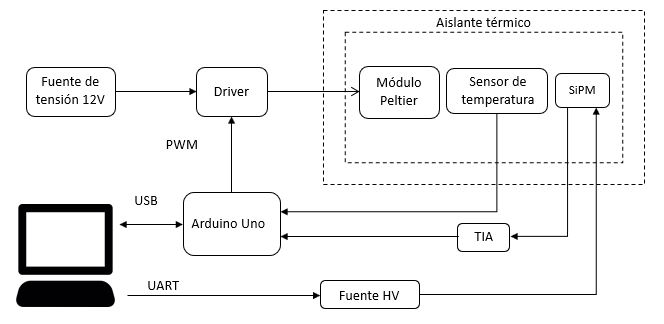
\includegraphics[width=0.6\textwidth]{Images/Sistema_Completo_ruptura}
  \label{fig:complete_system}
  \par\end{centering}
\end{figure}

%%%%%%%%%%%%%%%%%%%%%%%%%%%%%%%%%%%%%%%%%%%%%%%%%%%%%%%%%%%%%%%%%%%%%%%%%%%%%%%%%%%%%
\subsection{Control de temperatura.}
El sistema de control de temperatura está compuesto por tres partes principales que se muestran en la fig. \ref{fig:Temp_system} y son descritas a continuación: un módulo Peltier encargado de disipar y generar calor en función de la temperatura objetivo, un microcontrolador Atmega 328P en el cual se implementa el controlador PID y  un puente H como interfaz entre el sistema de control y el sistema de potencia, permitiendo controlar la magnitud y la dirección de la corriente entregada a las celdas Peltier.
\begin{figure}[h!]
\begin{centering}
    \caption{Sistema de control de temperatura. El parte superior se encuentra la caja oscura donde se ubica el SiPM, debajo están ubicadas las celdas Peltier junto a dos disipadores de calor y en la caja de aluminio se encuentra el puente H.}
    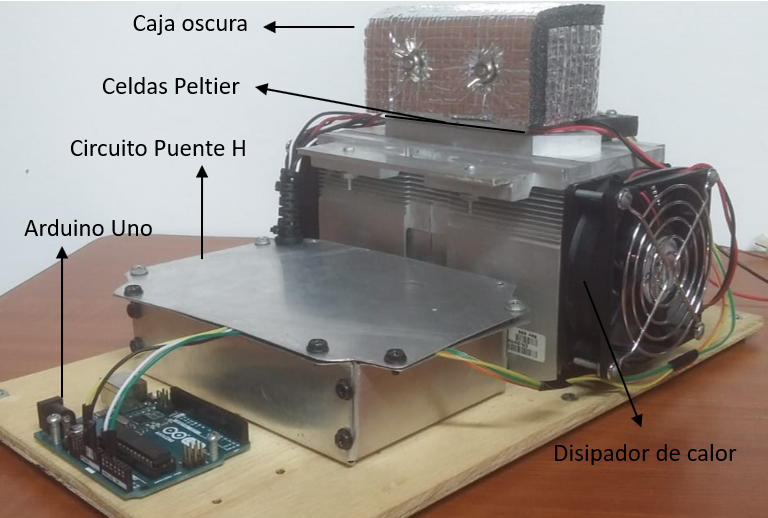
\includegraphics[width=0.6\textwidth]{Images/Sistema_termico}
    \label{fig:Temp_system}
  \par\end{centering}
\end{figure}
%%%%%%%%%%%%%%%%%%%%%%%%%%%
\subsubsection{Módulos Peltier.}
Su principio de funcionamiento es el efecto Peltier, descubierto en $1834$ por el físico francés Jean Charles Athanase Peltier, pero su aplicación práctica necesitó del desarrollo de los materiales semiconductores \citep{Sandoval2007}. Este efecto se caracteriza por la absorción o producción de calor en las caras de un semiconductor cuando una corriente eléctrica directa fluye a través de éste. \\ \\
Una celda Peltier está compuesta por  dos semiconductores con dopaje diferente (tipo-N y tipo-P) y una placa metálica entre estos. La dirección de la corriente eléctrica determina si el área se calienta o se enfría \citep{peltier_theory}, el calor generado mediante este efecto por unidad de tiempo está determinado por:
\begin{equation}
Q_{Pe}=(\Pi_{A}-\Pi_{B})\cdot I,
\label{peltier_eq}
\end{equation}
donde, $\Pi_{(A,B)}$ son los coeficientes Peltier de cada semiconductor e $I$ es la corriente eléctrica.\\ \\
La figura \ref{fig:celda} muestra la estructura interna de una Celda Peltier, donde se observa la configuración de los semiconductores y la absorción o producción de calor en función de la dirección de la corriente eléctrica a través de la celda.\\ \\
Para este trabajo se utilizó una celda Peltier TEC1-12706 \citep{datasheet_Peltier}. Sus parámetros son los siguientes: tensión máxima de $16.4~\mbox{V}$, corriente máxima de $6.4~\mbox{A}$, máxima capacidad de disipación de potencia 57 W y una máxima diferencia de temperatura entre la cara fría y la caliente de 75 $^\circ \mbox{C}$.

\begin{figure}[h!]
\begin{centering}
    \caption{Estructura interna de una celda Peltier. La dirección de la corriente (flecha roja) determina cuál de las caras absorbe o genera calor. Imagen adaptada de \citep{tesis_caract_SIPM}.}
    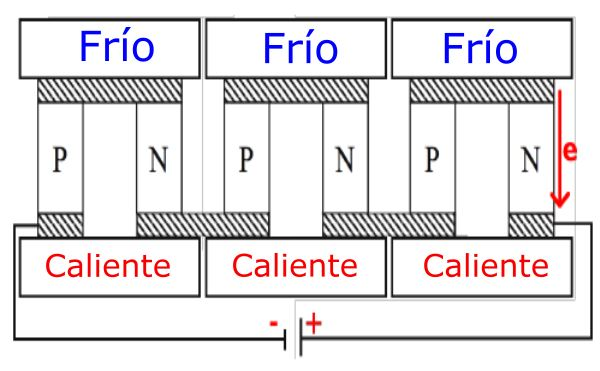
\includegraphics[width=0.45\textwidth]{Images/celda.JPG}
    \label{fig:celda}
  \par\end{centering}
\end{figure}

%%%%%%%%%%%%%%%%%%%%%%%%%%%
\subsubsection{Driver IR2110.}
Para realizar el control de temperatura en el SiPM, es necesario controlar la magnitud y la dirección de la corriente que se le suministra a las celdas Peltier, por eso se utiliza  el microcontrolador Atmega 328P para generar una señal de control PWM dependiendo de la temperatura objetivo. No obstante, la señal de control no puede ser conectada directamente a los MOSFET de potencia que se utilizan en el puente H, debido a que el voltaje $V_{GS}$ necesario para que el MOSFET opere en la región de saturación y suministre la corriente necesaria a la carga (6 A) es del orden de 12 V. Por este motivo, es indispensable implementar un \textit{driver}; es decir, un circuito que realiza la conversión de los 5 V suministrados por el microcontrolador a los 12 V necesarios para que los MOSFET del puente H operen correctamente, en este caso se utilizó el chip IR2110.
\begin{figure}[h!]
\begin{centering}
    \caption{Driver IR2110, utilizado para controlar el puente H por medio del microcontrolador Atmega 328P.}
    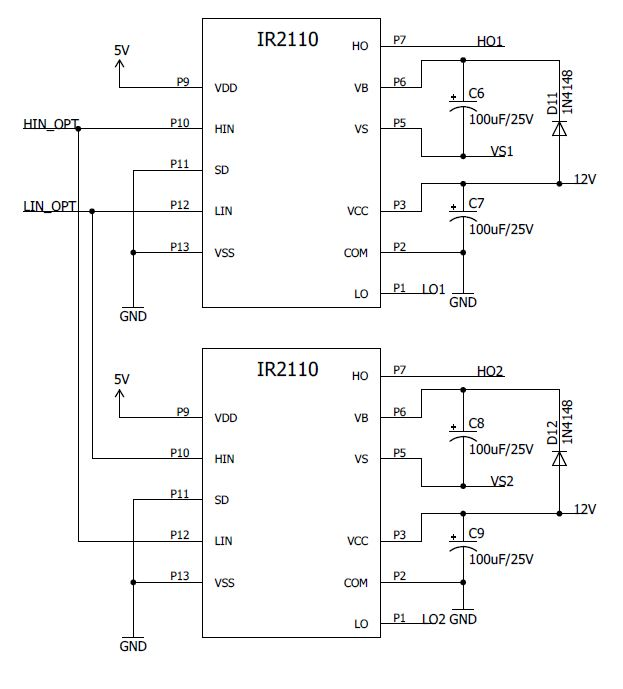
\includegraphics[width=0.6\textwidth]{Images/Driver.JPG}
    \label{fig:Driver}  
  \par\end{centering}
\end{figure}
\\ \\
El \textit{ International Rectifiers IR2110 driver}, es un driver de alta velocidad que puede entregar voltajes en el rango de los 10-20 V y puede soportar  corrientes de salida de hasta 2 A, mientras que entradas se adecuan para niveles de voltaje lógicos (TTL). En la figura \ref{fig:Driver}  se muestra la configuración utilizada y se puede observar que cada IR2110 controla medio puente H.\\ \\
El análisis del circuito  lo reduciremos únicamente a un IR2110, debido a que son dos circuitos iguales los que controlan el puente H completo. En la parte superior de la figura \ref{fig:Driver} se observa el circuito \textit{bootstrap}, el cual está compuesto por C6 y D11. Su funcionamiento es el siguiente: cuando HIN está en bajo y LIN está en alto, la señal activa la parte baja del puente H (transistor Q2), conectando VS1 a tierra y haciendo que C6 se cargue a través de D11 hasta el voltaje VB. Por otra parte, cuando LIN está en bajo y HIN está en alto la carga almacenada en C6 es utilizada para suministrar el voltaje que hace que el transistor Q1 se active.\\
%%%%%%%%%%%%%%%%%%%%%%%%%%%
\subsubsection{Puente H.}
\begin{figure}[h!]
\begin{centering}
    \caption{Puente H utilizado para controlar la magnitud y la  dirección de la corriente entregada a las celdas Peltier.}
    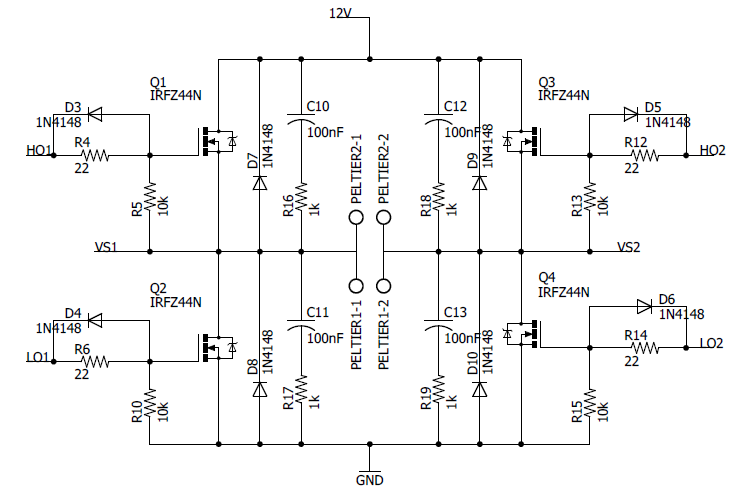
\includegraphics[width=0.8\textwidth]{Images/PuenteH.png}
    \label{fig:PuenteH}
  \par\end{centering}
\end{figure}
El circuito que aquí se emplea, es mostrado en la fig.  \ref{fig:PuenteH}. Inicialmente, mientras Q2  y Q3 permanecen inactivos, Q1 y Q4 se activan simultáneamente para suministrar a las celdas peltier un voltaje entre 0 y 12 V en función del ciclo útil de la señal PWM que activa los MOSFET. De esta forma se activa medio puente H y las celdas Peltier comienzan a refrigerar el interior de la caja donde se encuentra el SiPM. En caso contrario, cuando se activa la otra mitad del puente H controlado por Q2 y Q3 se cambia el sentido de la corriente y las celdas Peltier comienzan a calentar el interior de la caja.\\ \\
Asimismo, los diodos D3, D4, D5 y D6 permiten descargar rápidamente la  capacitancia de puerta de los MOSFET. Por otra parte, las resistencias R4, R6, R12 y R14 limitan la corriente en la puerta del transistor. Además, las resistencias R5, R10 R13 y R15 actúan como resistencias de \textit{pull-down} aterrizando la puerta del MOSFET cuando se encuentra inactivo, evitando dejar en la puerta un voltaje flotante que pueda activar el MOSTET. Finalmente, los diodos D7, D8, D9 y D10 son protección contra voltajes inversos, R16, R17, R18, R19, C10, C11, C12 y C13 son  una red \textit{snubber} de tensión RC para ayudar a la conmutación de los MOSFET y suprimir los picos de voltaje. 
\begin{figure}[h!]
\begin{centering}
  \caption{Implementación del puente H con los Drivers y demás circuitos necesarios para controlar la corriente que alimenta las celdas Peltier.}
  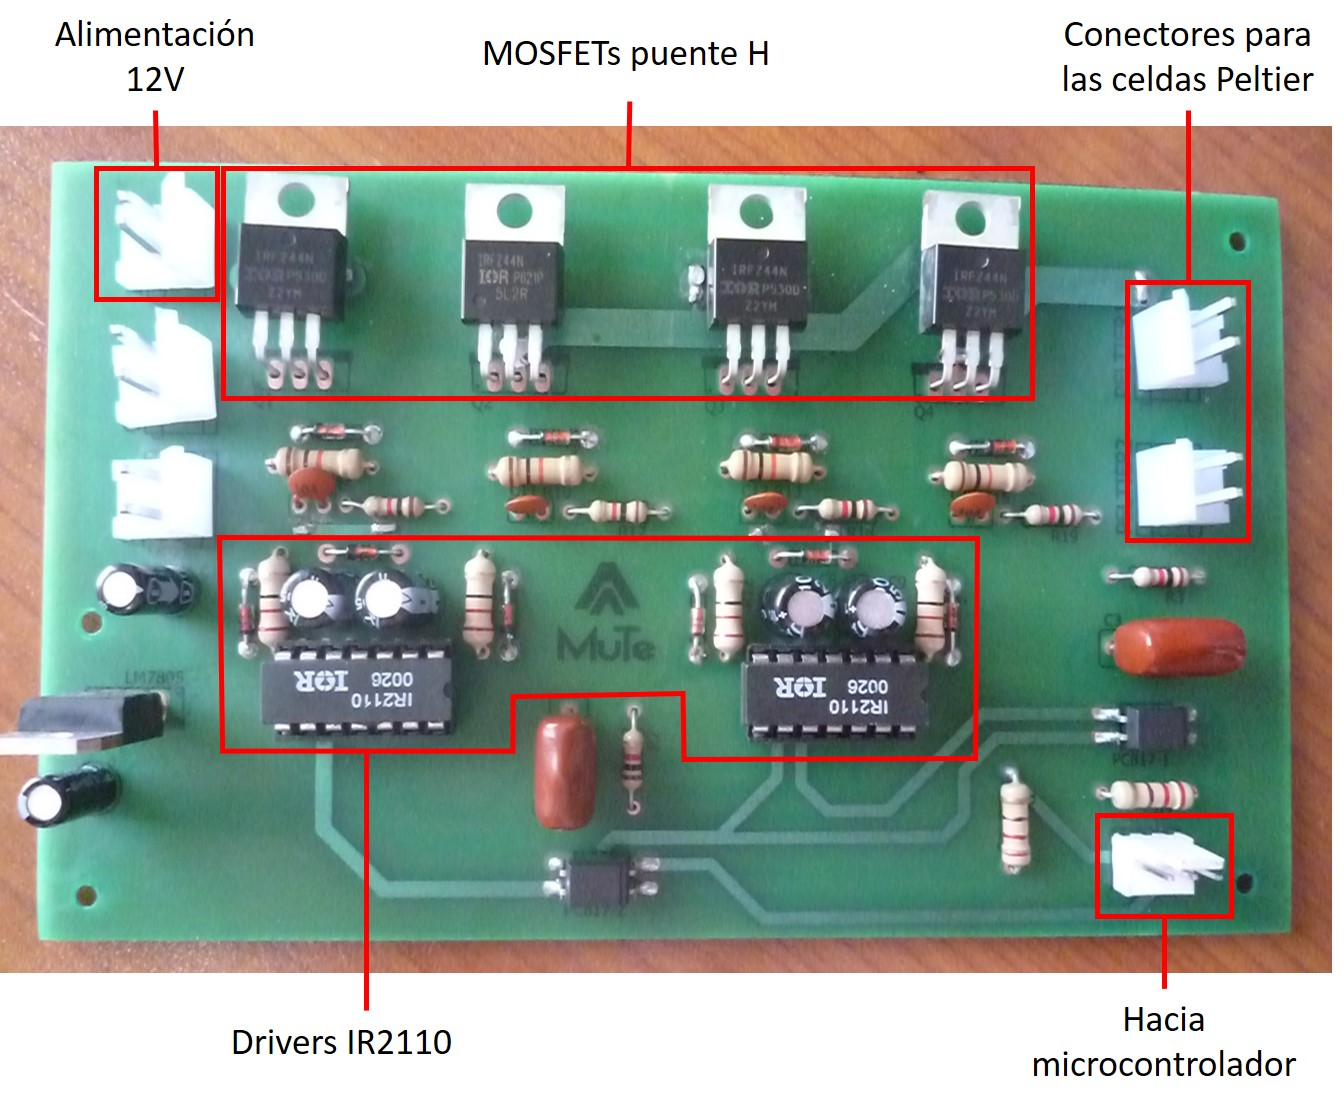
\includegraphics[width=0.6\textwidth]{Images/Tarjeta.jpg}
  \label{fig:PCB}
  \par\end{centering}
\end{figure}
%%%%%%%%%%%%%%%%%%%%%%%%%%%%
\subsubsection{Optoacoplamiento.}
Como punto de partida, es necesario proteger las salidas del microcontrolador, por esta razón se utilizó un optoacoplador PC817, el cual consiste en un Diodo Emisor Infrarojo (IRED) que está acoplado a un fototransistor. En este caso, los pines 1 y 2 están conectados a las salidas del microcontrolador, mientras que el pin 3 está conectado a la entrada del driver IR2110. En este circuito, las resistencias R1 y R2 limitan la corriente que pasa por el IRED y por el fototransitor respectivamente, mientras que C2 ayuda a eliminar oscilaciones en el voltaje debido transitorios de conmutación. 
\begin{figure}[h!]
\begin{centering}
    \caption{Optoacopladores utilizados para asilar eléctricamente las salidas del microcontrolador y las entradas del driver.}
    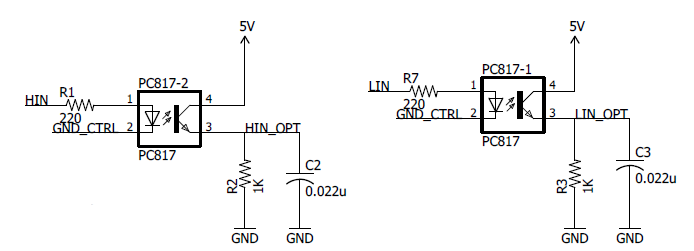
\includegraphics[width=0.7\textwidth]{Images/Optoacoplador.png}
    \label{fig:optoacoplador}
  \par\end{centering}
\end{figure}
%%%%%%%%%%%%%%%%%%%%%%%%%%%%%
\subsubsection{Regulador de voltaje.}
Para la polarización del optoacoplador y el nivel de referencia del voltaje  VDD del driver IR2110, fue necesario utilizar un regulador de voltaje LM7805, que a partir de 12 V permite obtener los 5 V necesarios. La topología básica, que se muestra en la fig.  \ref{fig:Regulador} la suministra el fabricante en una nota  de aplicación. 
\begin{figure}[h!]
\begin{centering}
    \caption{Regulador de voltaje LM7805 utilizado para obtener los 5 V necesarios para polarizar en optoacoplador y suministrar el nivel de voltaje lógico de referencia al driver IR2110.}
    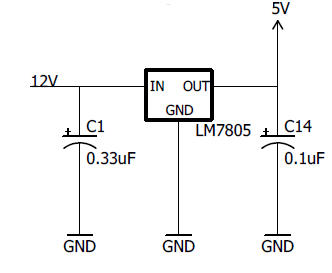
\includegraphics[width=0.35\textwidth]{Images/Regulador.png}
    \label{fig:Regulador}
  \par\end{centering}
\end{figure}
%%%%%%%%%%%%%%%%%%%%%%%%%%%%%%
\subsubsection{Sensor de temperatura.}
El LM35 es un sensor de temperatura de precisión, su salida de voltaje es linealmente proporcional a la temperatura, con una exactitud es de $ \pm 0.3 ~^\circ \mbox{C}$. Su función de transferencia está dada por:
\begin{equation}
    V_{out}=10~\mbox{mV}/^\circ \mbox{C} \times~T,
    \label{SensorTf}
\end{equation}
donde, $V_{out}$ es el voltaje de salida del sensor LM35 y $T$ es la temperatura en $^\circ \mbox{C}$.\\ \\
Por otra parte, en al figura \ref{fig:TempSense} se muestra la topología utilizada para que el sensor de temperatura LM35 proporcione una salida en el rango de $-55~a ~150~ ^\circ$C. 
\begin{figure}[h!]
\begin{centering}
    \caption{Circuito utilizado para que el sensor de temperatura LM35 funcione en su rango completo $-55~a ~150~ ^\circ \mbox{C}$.}
    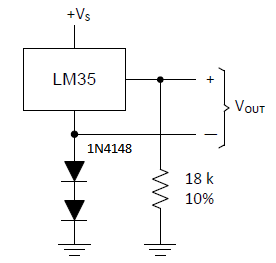
\includegraphics[width=0.3\textwidth]{Images/TempSensor.png}
    \label{fig:TempSense}
  \par\end{centering}
\end{figure}
\\ \\
El sensor de temperatura se ubicó dentro de la caja oscura, como se muestra en la fig. \ref{fig:insideBox}, muy cerca del SiPM con el fin de tener la menor diferencia de temperatura entre estos.
\begin{figure}[h!]
\begin{centering}
    \caption{Ubicación del sensor de temperatura y del SiPM dentro de la caja oscura del sistema de control de temperatura.}
    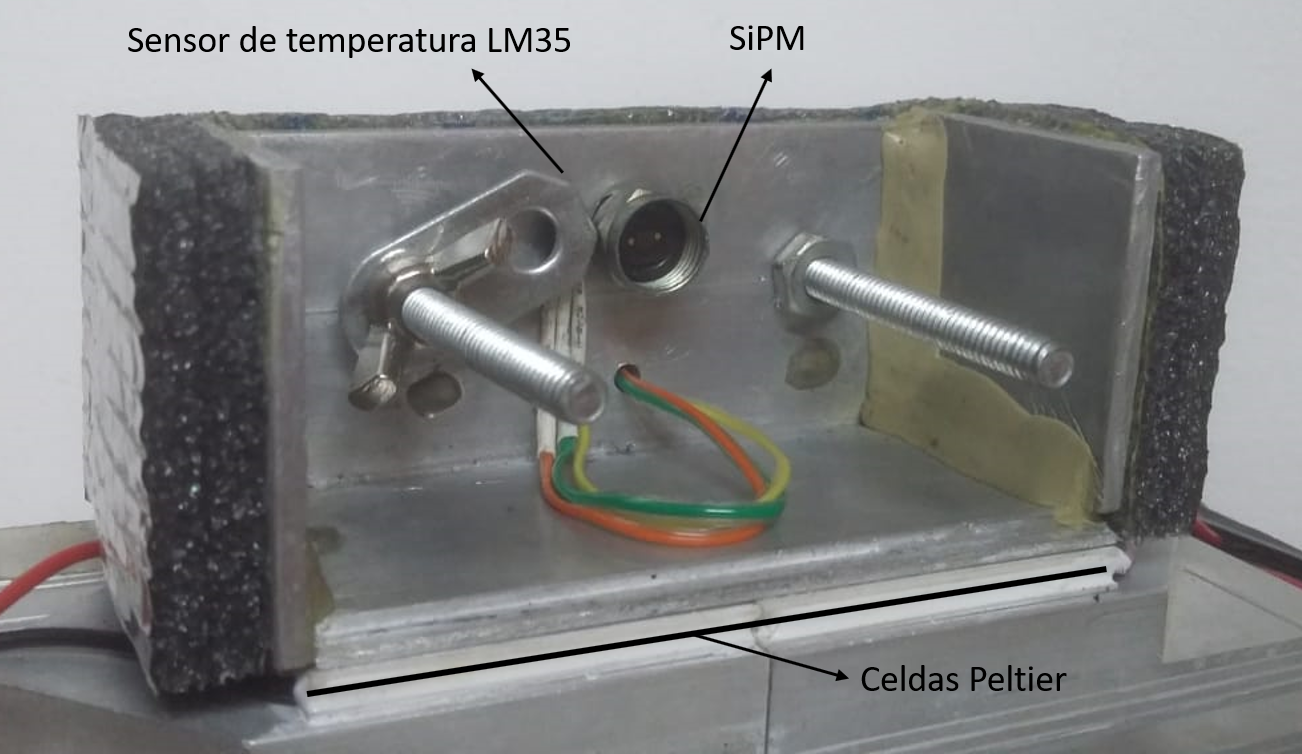
\includegraphics[width=0.5\textwidth]{Images/InsideBox.png}
    \label{fig:insideBox}
  \par\end{centering}
\end{figure}
%%%%%%%%%%%%%%%%%%%%%%%%%%%%%%%%
\subsubsection{Microcontrolador Atmega 328P.}
% \begin{figure}[h!]
% \begin{centering}
%   \includegraphics[scale=0.7]{Images/Arduino.JPG}
%     \caption{Tarjeta Arduino Uno utilizada para la implementación del controlador PID, realizar la acción de control y el monitorio de la temperatura al interior de la caja donde se ubica el SiPM  .}
%     \label{fig:Arduino}
%   \par\end{centering}
% \end{figure}
Este microcontrolador tiene 14 pines digitales de entrada-salida (de los cuales 6 pueden ser utilizados como PWM), 6 entradas analógicas, un cristal de 16 MHz y conexión USB. La función del microcontrolador en el sistema de control es realizar la lectura del sensor de temperatura y calcular el error entre este valor y la temperatura establecida como objetivo, para finalmente, aplicar el algoritmo (controlador PID)\footnote{https://github.com/juanvillafrades/Caracterizacion-SiPMs/blob/master/PID\_control.ino} necesario para para estabilizar la temperatura en su valor objetivo.   

%%%%%%%%%%%%%%%%%%%%%%%%%%%%%%%%
\subsubsection{Sistema FOPDT.}
Un FOPDT ( First Order Plus Dead Time) es un modelo dinámico ampliamente utilizado para la obtención de los parámetros de sintonización de un controlador PID, su función de transferencia está dada por:
\begin{equation}
Gp(s)=  \frac{k\cdot e^{-Ls}}{1+Ts},
\label{FOPDT_model}
\end{equation}
donde, $k$ es la ganancia en estado estable de la planta, $T > 0$  representa la constante de tiempo de la planta y $L > 0$ es el tiempo muerto. En este caso, se utilizó un modelado de \textit{caja negra}, el cual se emplea cuando no se conocen todos los parámetros físicos del sistema. En lo que respecta al método, este consiste en registrar los datos de la salida del sistema cuando es estimulado  con una señal conocida.\\ \\
Al respecto, la descripción del procedimiento se muestra en la fig. \ref{fig:Modelo_caja_negra}, donde se observa que el sistema se estimula con una señal de tipo escalón unitario, mientras se registra la temperatura en el interior de la caja, esto corresponde con la señal de salida del sistema. Además, mediante el uso de la \textit{System idetification toolbox} de Matlab\textsuperscript \textregistered $~$se identificaron las funciones de transferencia de la planta.
\begin{figure}[h!]
\begin{centering}
    \caption{Sistema de control de temperatura compuesto por un puente H, dos celdas Peltier y un sensor de temperatura, con una entrada de tipo escalón unitario.}
    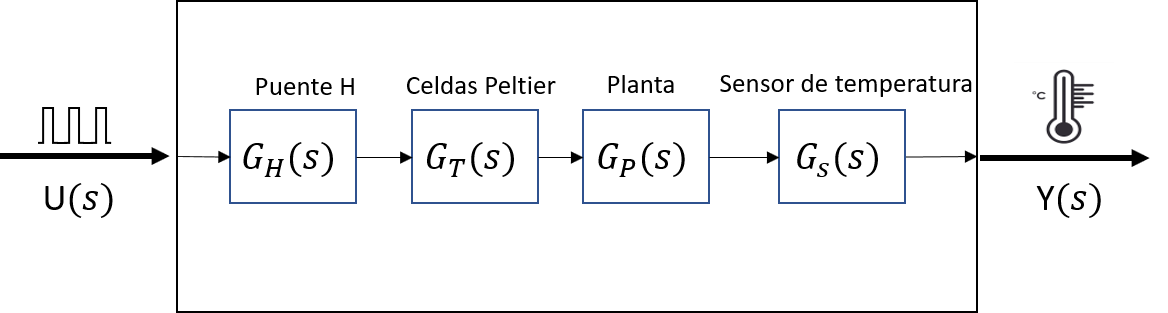
\includegraphics[width=0.7\textwidth]{Images/Modelo_caja_negra.png}
    \label{fig:Modelo_caja_negra}
  \par\end{centering}
\end{figure}
\\ \\
Para la caracterización del sistema en modo refrigeración se utilizó una señal de entrada de tipo PWM con un ciclo útil del $100\%$ que corresponde con un voltaje de alimentación en las celdas Peltier de $12$ V y se registró la temperatura al interior de la caja durante 10 minutos, como se muestra en la cruva azul de la fig. \ref{fig:step_response}. Por otra parte, para la caracterización del sistema en modo calentamiento, la señal PWM utilizada tenía un ciclo útil del  $37\%$ correspondiente a un voltaje de alimentación en las celdas Peltier de $4.6~\mbox{V}$, su resultado se muestra en la curva naranja de la fig. \ref{fig:step_response}. Nótese que para el calentamiento no se utilizó el máximo ciclo útil debido a  que su efecto sobre el sistema es mucho más agresivo.
\begin{figure}[h!]
\begin{centering}
    \caption{Respuestas del sistema a una entrada de tipo escalón. La curva azul corresponde a la  refrigeración y la naranja al calentamiento. En la forma de las curvas se puede observar tanto el retardo temporal como la forma exponencial de la respuesta en un sistema de primer orden.}
  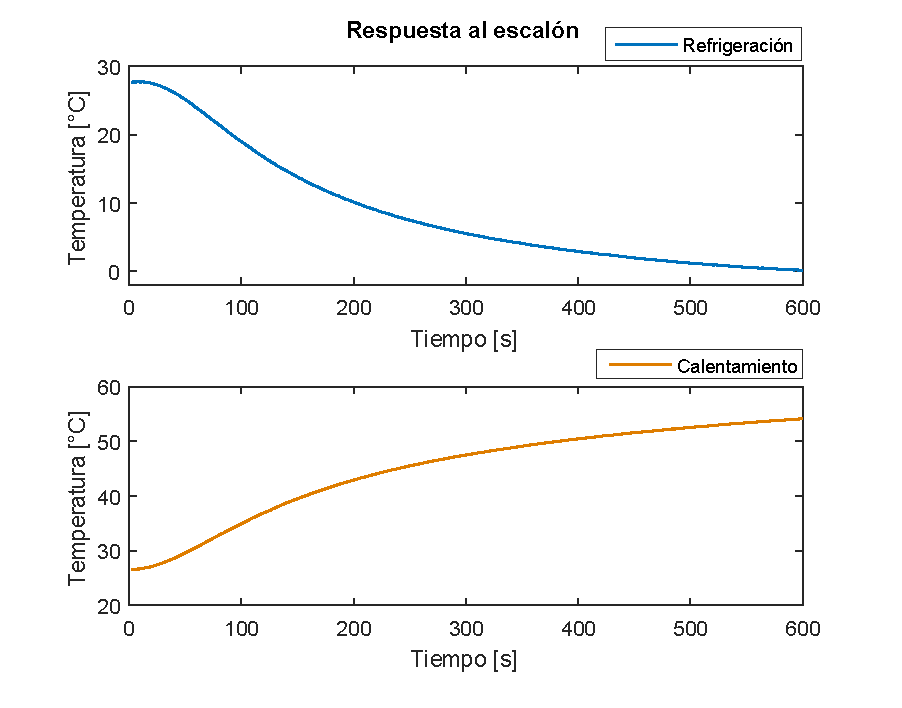
\includegraphics[width=0.7\textwidth]{Images/plant_response.eps}
    \label{fig:step_response}
  \par\end{centering}
\end{figure}
\begin{figure}[h!]
\begin{centering}
    \caption{Respuestas del modelo FOPDT del sistema a una entrada de tipo escalón. La curva azul corresponde a la  refrigeración y la naranja al calentamiento.}
  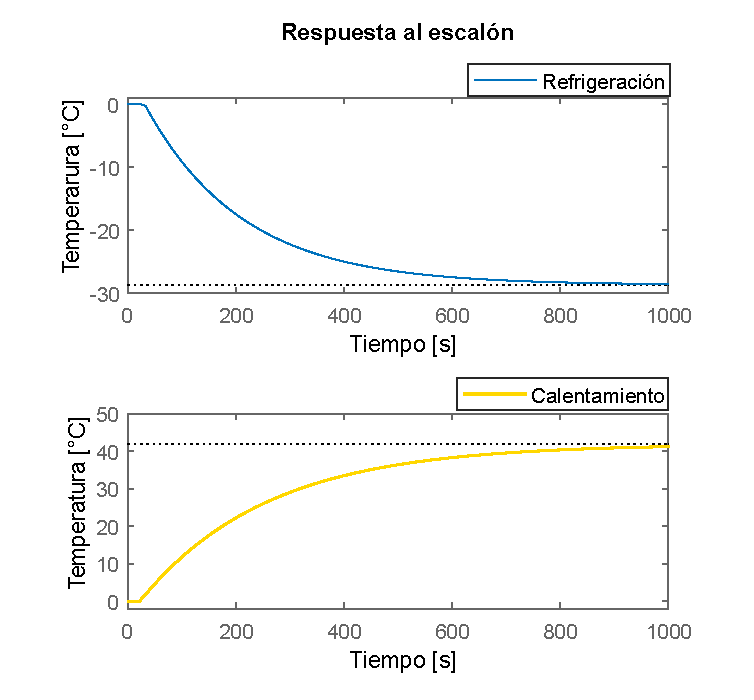
\includegraphics[width=0.7\textwidth]{Images/step}
    \label{fig:step_model_plant}
  \par\end{centering}
\end{figure}
\\ \\
Para obtener los modelos dinámicos del sistema, a partir de los datos de entrada-salida registrados, se realizó un preprocesamiento que consistió en eliminar el \textit{offset}. Posteriormente, con la ayuda de Matlab\textsuperscript \textregistered $~$se identificaron los FOPDT del sistema, la función de transferencia para la refrigeración $G_{p1}(s)$ se muestra en la ecuación \ref{tf_cooling} y para el calentamiento $G_{p2}(s)$ es la ecuación \ref{tf_heating}.
\begin{equation}
G_{p1}(s)=  \frac{-29.02\cdot e^{-27.92 s}}{1+187.27 s},
\label{tf_cooling}
\end{equation}
\begin{equation}
G_{p2}(s)=  \frac{29.31\cdot e^{-23.92 s}}{1+215.96 s}.
\label{tf_heating}
\end{equation}
Con estas funciones de transferencia se graficó la respuesta del sistema ante una entrada de tipo escalón. Este resultado se muestra en la figura \ref{fig:step_model_plant} donde el ajuste de los modelos FOPDT y los datos es de un $97\%$.
%%%%%%%%%%%%%%%%%%%%%%%%%%%%%%%%%
\subsubsection{Controlador PID.}
\begin{figure}[h!]
\begin{centering}
    \caption{Diagrama de bloques del sistema de control de temperatura.}
    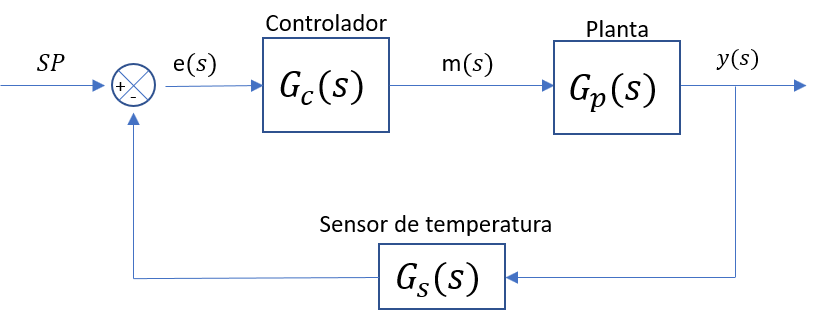
\includegraphics[width=0.6\textwidth]{Images/DiagramaOnOff.png}
    \label{fig:DiagramaOnOff}
  \par\end{centering}
\end{figure}
Para mantener estable la temperatura dentro de la caja que contiene el SiPM fue necesario realizar un control de temperatura. Como primera aproximación se implementó un control On-Off, este tipo de control es muy común en sistemas de control de temperatura, se caracteriza por contar únicamente con dos estados (encendido o apagado) y consiste en activar la acción de control (señal PWM) cuando la variable controlada (temperatura) está por arriba del valor deseado (set point) y luego desactivarlo cuando esté por debajo. La función de trasferencia utilizada en la implementación del control se muestra en la ecuación \ref{OnOff_eq} 
\begin{equation}
  m(t) = \left \{ \begin{matrix} u_{1}(t) & \mbox{si }e(t) \ge 0,
\\u_{2}(t) & \mbox{si }e(t) < 0, \end{matrix}\right.
\label{OnOff_eq}
\end{equation}
donde, $u_{1}(t)$ es la función escalón que representa una señal PWM con un ciclo útil de $100\%$ y hace que las celdas Peltier funcionen en modo refrigeración. Por otra parte, $u_{2}(t)$ es una función escalón que representa una señal PWM con un ciclo útil de $37\%$ y hace que las celdas Peltier funcionen en modo calentamiento. 
\begin{figure}[h!]
\begin{centering}
    \caption{Respuesta del sistema con un controlador On-Off cuando se establece una temperatura objetivo de $5~^\circ \mbox{C}$. Esta respuesta presenta oscilaciones con un amplitud de $4.9~^\circ \mbox{C}$.}
  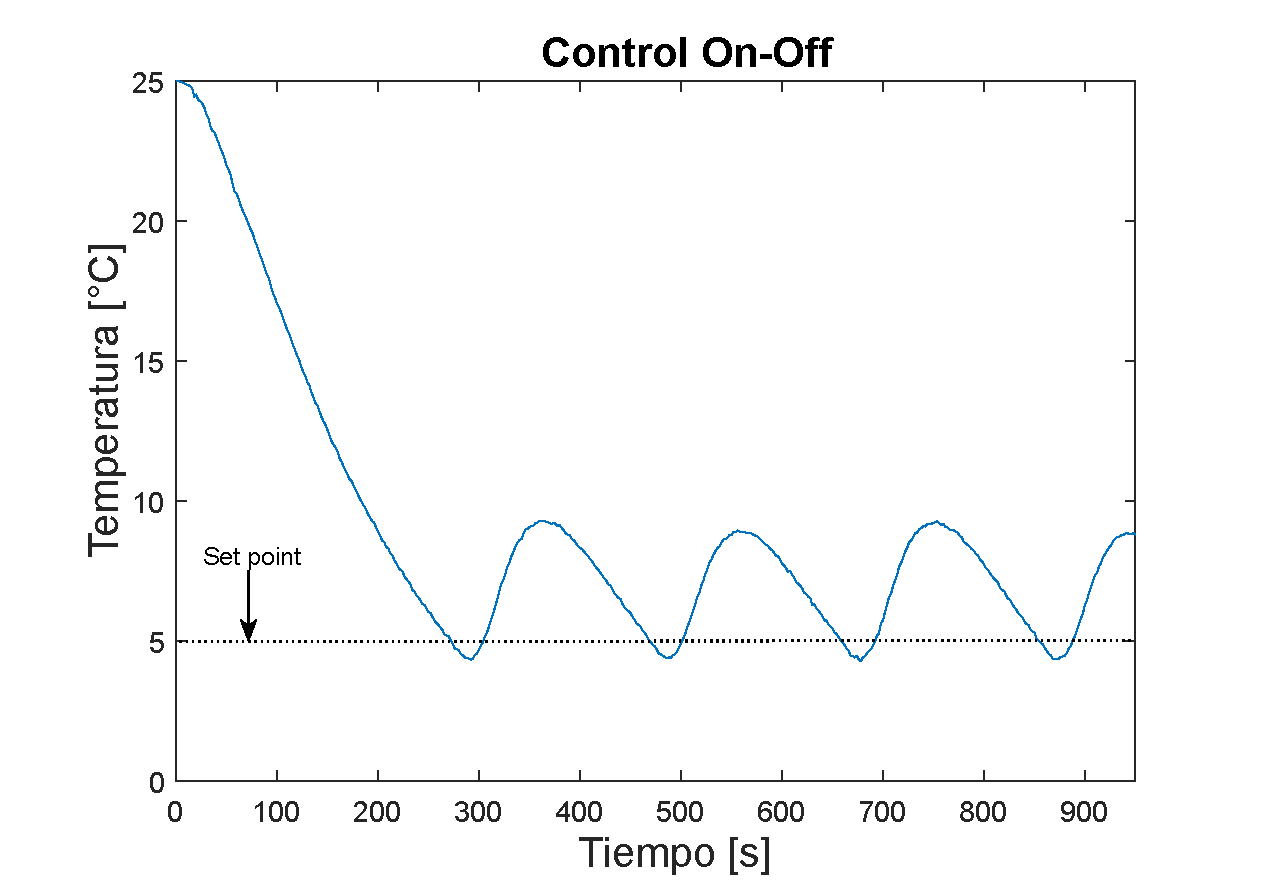
\includegraphics[width=0.6\textwidth]{Images/ControlOnOff.eps}
    \label{fig:ControlOnOff}
  \par\end{centering}
\end{figure}
\\ \\
En la figura \ref{fig:ControlOnOff} se muestra el resultado de la implementación del control On-Off. Se puede observar como el sistema llega a su temperatura objetivo en $270$ segundos y a partir de este punto comienza a realizar oscilaciones con una brecha diferencial de $4.9~^\circ \mbox{C}$. Esto representa un rango de variación muy amplio y hace que este tipo de controlador no sea la mejor opción para este caso. Por lo tanto, se plantea la necesidad de implementar un controlador de tipo Proporcional Integral Derivativo.\\ \\
El controlador  Proporcional Integral Derivativo (PID) es el algoritmo de control más implementado en automatización de procesos industriales \citep{Astrom}. Este  utiliza el principio de realimentación, que consiste en comparar la salida del sistema con un nivel de referencia y emplear esta diferencia para realizar una acción de control. Este tipo de realimentación se denomina realimentación negativa porque la variable manipulada es opuesta a la variable del proceso. Es decir, cuando la variable del proceso es mucho más pequeña que el punto de ajuste se incrementa la variable manipulada, mientras que cuando la variable del proceso es más grande que el punto de ajuste se disminuye la variable manipulada. Entre sus principales ventajas se encuentra el hecho de hacer que la variable  de proceso se acerque al punto de ajuste,  incluso ante perturbaciones y variaciones.\\ \\
Un controlador PID, cuenta con tes partes principales: en primer lugar, una parte proporcional que consiste en el producto entre el error $e(t)$ y la constante proporcional $k_P$. Este término define la rapidez con que la salida del sistema se acerca al punto de ajuste; pero, para valores muy grandes de $k_P$, hace que la salida del sistema oscile y presente grandes sobreimpulsos.
$$
u_P(t)=k_{P}\cdot e(t).  
$$
En segundo lugar, una parte integral que se encarga de eliminar el error en estado estable agregado por el término proporcional. El control integral actúa cuando hay una diferencia entre la variable del proceso y el punto de ajuste, realizando la sumatoria de esta diferencia en el tiempo y agregándola a la acción proporcional.\\
$$
u_I(t) = k_{I}\int_{0}^{t}{e(t)dt}.
$$
Finalmente, el término derivativo mejora la estabilidad del lazo cerrado, permitiendo que el sistema reaccione rápidamente ante un cambio en el error.\\

$$
u_D(t) = k_{D}\frac{d}{dt}e(t).
$$
El controlador  PID completo está compuesto por la suma de los términos anteriormente mencionados.
\begin{eqnarray}
u_{PID}(t) & = & u_P(t) + u_I(t) + u_D(t); \\
u_{PID}(t) & = & k_{P}\cdot e(t) + k_I\int_{0}^{t}{e(\tau)d\tau} + k_{D}\frac{d}{dt}e(t).
\label{PID_continuo}
\end{eqnarray}\
Para implementar el controlador PID en un microcontrolador es necesario discretizar  la expresión \ref{PID_continuo}. Utilizando la aproximación rectangular hacia atrás se puede obtener la versión discreta de los términos integral y derivativo.\\
La acción proporcional discreta es:
$$
u_P(k)=k_{P}\cdot e(k).  
$$\
La acción derivativa discreta es:
$$
u_D(k) = k_{D}\frac{e_k-e_{k-1}}{T_s}.
$$
La acción integral discreta es:
$$
u_I(k) =  k_{I}\cdot \displaystyle\sum_{i=1}^{k} e_{i}T_s.
$$
Realizando la suma de estas acciones discretas se obtiene la expresión para el controlador PID discreto.\\

\begin{equation}
 u_{PID}(k) = k_{P}\cdot e(k) + k_{I} \displaystyle\sum_{i=1}^{k} e_{i}T_s + k_{D}\frac{e_k-e_{k-1}}{T_s}.
\label{pid_eq}
\end{equation}
El principal parámetro que se debe determinar para poder implementar este controlador discreto es el periodo de muestreo ($T_s$). En la práctica existe un criterio para determinar este valor y está dado por la siguiente expresión:
$$
T_s < \frac{T}{10} ~,
$$
donde, $T$ representa la constante de tiempo del sistema. Como se puede observar en las ecuaciones \ref{tf_cooling} y \ref{tf_heating} de los modelos del sistema, tanto para la refrigeración como para el calentamiento, estas constantes son  $187.27$ s y $215.96$ s respectivamente. Tomando el peor de los casos, es decir, la constante de tiempo del sistema para la refrigeración, se obtiene:
$$
T_s < \frac{187.27}{10} ~\mbox{s} = 18.727 ~\mbox{s}.\\
$$
% $$
% T_s < 18.727 ~\mbox{s} \\
% $$
Teniendo en cuenta el criterio anteriormente mencionado se eligió un periodo de muestreo de 2 s. \\ \\
La sintonización del controlador consiste en determinar los parámetros ($k_P, k_I~ \mbox{y}~ k_D$) que cumplan con los requerimientos de diseño establecidos para el sistema controlado. Así, existen diferentes métodos para realizar esta sintonización: métodos experimentales basados en datos obtenidos del proceso y métodos analíticos que se basan en el modelo matemático del sistema. \\ \\
En este caso se utilizó una aplicación de Matlab\textsuperscript \textregistered  $~$llamada \textit{PID tuner} que ofrece una interfaz desde donde se puede seleccionar el tipo de controlador que se desea implementar a partir del modelo matemático del sistema, también se pueden variar los parámetros del controlador mientras se observa gráficamente la respuesta en magnitud, fase y tiempo del sistema para elegir el conjunto de parámetros que cumplan los requerimientos del sistema de control.\\ \\
Para el sistema de calentamiento se obtuvieron los siguientes parámetros del controlador: $k_P= 11.058;~k_I= 0.044;~k_D=41.45$. Este conjunto de parámetros se seleccionaron teniendo en cuenta el tiempo de establecimiento del sistema, el sobre impulso y el tiempo pico.\\ \\
En la figura \ref{fig:Respuesta_PID_c} se muestra la respuesta del sistema en el tiempo para las temperaturas objetivo de $30$, $40$ \mbox{y} $50~^\circ \mbox{C}$ durante $10$ minutos. Adicionalmente, en la tabla \ref{table_PID_c} se muestran los principales parámetros de respuesta del controlador para cada una de las temperaturas objetivo, donde se puede notar que el sistema logra establecerse en la temperatura objetivo en un tiempo menor a $534$ segundos, presentado un máximo sobreimpulso del $37,2\%$.
\begin{figure}[h!]
\begin{centering}
    \caption{Respuesta del sistema de calentamiento con un controlador PID para temperaturas objetivo de 30 $^\circ $C (curva azul), 40 $^\circ $C (curva amarilla) y 50 $^\circ $C (curva roja).}
    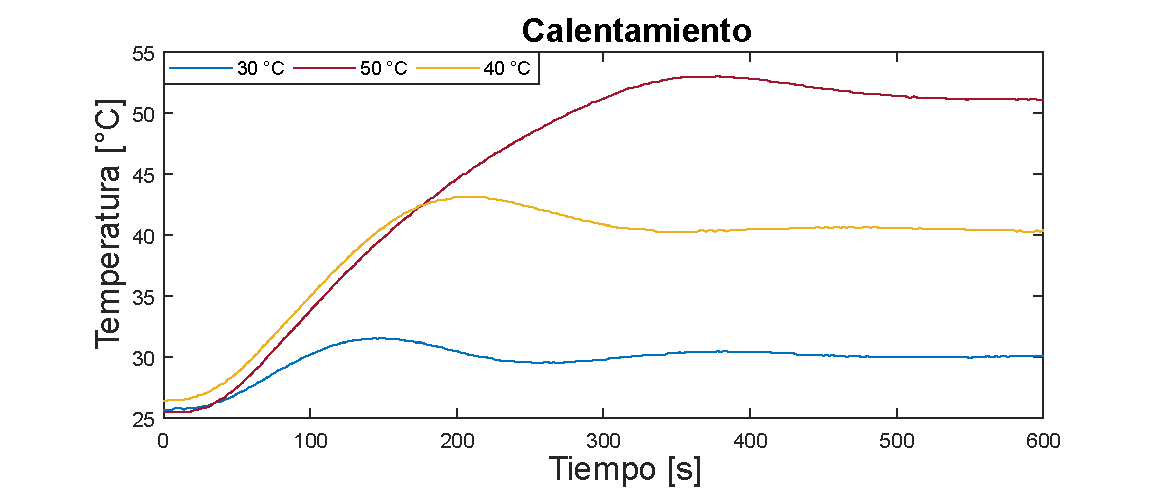
\includegraphics[width=0.7\textwidth]{Images/PID_calentamiento.eps}
    \label{fig:Respuesta_PID_c}
  \par\end{centering}
\end{figure}
\\ \\
Para calcular los parámetros de respuesta del controlador se tuvo en cuenta la temperatura inicial y para el tiempo de establecimiento ($t_s$) se utilizó el criterio del $5\%$, que define que este tiempo es el tiempo que tarda el sistema en encontrarse dentro del rango de  $\pm5\%$ de la temperatura objetivo. Para este caso a la temperatura objetivo se le debe restar la temperatura inicial (temperatura ambiente). El tiempo pico ($t_p$) se determinó como el tiempo en que el sistema llega a su valor máximo. El porcentaje de sobreimpulso ($O.S$) se calculó utilizando la expresión \ref{overshoot_ec}.\\ 
\begin{eqnarray}
    M_p&=& y_{max} - y_{ss},\\
    O.S&=&\frac{M_p}{y_{ss}-y_0}\times100\%,
    \label{overshoot_ec}
\end{eqnarray}
donde, $M_p$ corresponde al máximo sobreimpulso, $y_{max}$ es el valor máximo de temperatura, $y_{ss}$ es el valor de temperatura es estado estable y $y_0$ es el valor inicial de temperatura ($\sim26~^\circ \mbox{C}$).
\begin{table}[htbp]
\caption{Parámetros de respuesta del controlador en modo calentamiento para diferentes temperaturas objetivo.}
    \label{table_PID_c}
	\centering
	\begin{tabular}{ c  c  c c}
    \hline
    Set point [$~^\circ \mbox{C}$]       & $t_s [\mbox{s}]$    & $t_p[\mbox{s}]$     &  $O.S[\%]$    \\ \hline
    \multicolumn{1}{c}{30}      & $432$        & $136$        & $37,2$    \\
    \multicolumn{1}{c}{40}      & $310$        & $200$        & $21.4$   \\
    \multicolumn{1}{c}{50}      & $534$        & $378$        & $12.2$   \\ \hline
	\end{tabular}
\end{table}
\\ \\
Para el sistema de refrigeración se realizó el mismo proceso de sintonización utilizado en el sistema de calentamiento y se obtuvieron los siguientes parámetros del controlador: $k_P= 30.6;~k_I= 0.148;~k_D=100$. En la figura \ref{fig:Respuesta_PID_e} se observa la respuesta en el tiempo del sistema para temperaturas objetivo de $0, 10 ~\mbox{y}~20~^\circ\mbox{C}$ durante 10 minutos. Así, el sistema logra estabilizarse en cada unos de los casos y los parámetros de respuesta del controlador se muestran en la tabla \ref{table_PID_e}, donde se puede concluir que el sistema presenta un máximo sobreimpulso del $26,6\%$, un tiempo pico máximo de $486$ segundos y un tiempo de establecimiento máximo de $576$ segundos.\\
\begin{figure}[h!]
\begin{centering}
    \caption{Respuesta del sistema de refrigeración con un controlador PID para temperaturas objetivo de 0 $^\circ $C (curva azul), 10 $^\circ $C (curva celeste) y 20 $^\circ $C (curva amarilla).}
    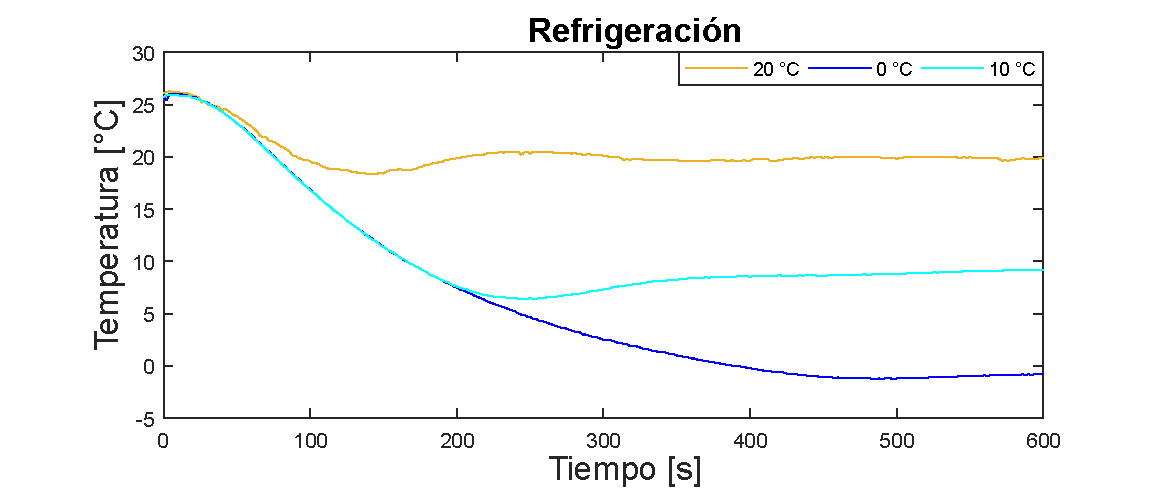
\includegraphics[width=0.7\textwidth]{Images/PID_enfriamiento.eps}
    \label{fig:Respuesta_PID_e}
  \par\end{centering}
\end{figure}

\begin{table}[h!]
\caption{Parámetros de respuesta del controlador en modo refrigeración para diferentes temperaturas objetivo.}
    \label{table_PID_e}
	\centering
%    \begin{threeparttable}
	\begin{tabular}{ c  c  c  c c}
    \hline
    Set point [$~^\circ \mbox{C}$]       & $t_s [\mbox{s}]$    & $t_p[\mbox{s}]$    &  $O.S[\%]$    \\ \hline
    \multicolumn{1}{c}{0}     & $342$        & $486$        & $5$    \\
    \multicolumn{1}{c}{10}      & $576$        & $244$        & $22,5$   \\
    \multicolumn{1}{c}{20}      & $402$        & $138$        & $26,6$   \\ \hline
	\end{tabular}	
%    \end{threeparttable}
\end{table}
%%%%%%%%%%%%%%%%%%%%%%%%%%%%%%%%%%%%%%%%%%%%%%%%%%%%%%%%%%%%%%%%%%%%%%%%%%
\subsection{Circuito de medición de corriente.}
El segundo módulo de medición para el proceso de caracterización del voltaje de ruptura es el circuito de medición de corriente. La corriente que se necesita medir es la corriente oscura del  SiPM, esta corriente es del orden de los nanoamperios (nA). Según \citep{low_level} existen dos técnicas muy utilizadas para realizar mediciones de corriente: medición en derivación o ``\textit{shunt}'' ~y medición mediante un amplificador de transimpedancia o amperímetro realimentado.
\begin{figure}[h!]
\begin{centering}
    \caption{Topología de amperímetro tipo ``\textit{shunt}''. }
    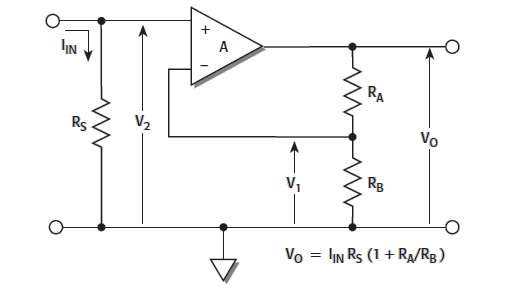
\includegraphics[width=0.5\textwidth]{Images/Shunt.png}
    \label{fig:shunt_circuit}
  \par\end{centering}
\end{figure}
\\ \\
De esta manera, la técnica de medición tipo ``\textit{shunt}'' consiste en poner una resistencia en serie con la fuente de corriente ($I_N$) que se desea medir, según la ley de Ohm. Esto genera una caída de voltaje ($V_2$) proporcional a la corriente que pasa por la resistencia ($R_s$), como se muestra en la fig. \ref{fig:shunt_circuit}. Sin embargo, el voltaje de entrada ($V_2$), también llamado voltaje de carga (\textit{Burden Voltage}), es una de las principales desventajas de esta topología. Si se necesita medir corrientes en el orden de los nanoamperios, entonces $R_s$ debe ser del orden de los M$\Omega$ para generar un voltaje de carga del orden de los mV.\\
La salida del amplificador no inversor se calcula como: 
\begin{eqnarray}
    V_o &=& V_2\left(1+\frac{R_A}{R_B}\right);\\
     V_o &=& I_{IN}R_s\left(1+\frac{R_A}{R_B}\right).
\end{eqnarray}
\begin{figure}[h!]
\begin{centering}
    \caption{Amperímetro de realimentación basado en un amplificador de transimpedancia  (TIA). }
    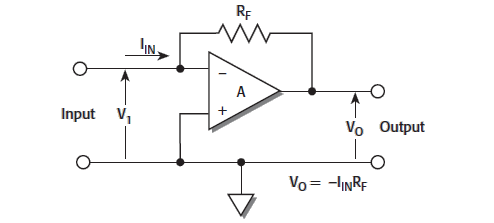
\includegraphics[width=0.6\textwidth]{Images/feedback.png}
    \label{fig:feedback_circuit}
  \par\end{centering}
\end{figure}
\\ \\
Por otra parte, la técnica de medición basada en un amplificador de transimpedancia consiste en hacer pasar la corriente de entrada ($I_{IN}$) por la resistencia de realimentación ($R_F$) de un TIA y generar un voltaje en la salida del amplificador que es una medida directa de la corriente de entrada, minimizando el voltaje de carga. \\ \\
El principal requisito de operación es que el valor de \textit{offset} de la corriente del amplificador debe ser mucho menor que la corriente $I_{IN}$ para que su efecto en la medición sea despreciable. Además, para altas frecuencias la capacitancia de salida de la fuente de corriente y la capacitancia de entrada del amplificador afectan la estabilidad del circuito. Para mitigar este efecto (compensar el amplificador) se debe utilizar un capacitor en paralelo con $R_F$.    
\begin{equation}
    V_o= -I_{IN} R_F.
\end{equation}{}
\\ \\
En este trabajo se utilizó la topología tipo ``\textit{shunt}'', debido a que las corrientes que se deben medir son generadas por un SiPM que  se polariza con un voltaje en el rango de los 40 a 60 V y el voltaje de carga que se genera utilizando la topología tipo ``\textit{shunt}'' es de máximo 500 mV.%, adicionalmente esta topología es típica en mediciones de precisión de corriente \citep{low_level}  y sumado a que uno de los objetivos de este trabajo es desarrollar estos módulos de medición con componentes de bajo costo y de fácil  acceso.
\begin{figure}[h!]
\begin{centering}
    \caption{Circuito utilizado para el amperímetro tipo ``\textit{shunt}''. Compuesto por cuatro etapas, una etapa de conversión de corriente a voltaje, un búfer, un amplificador inversor y un filtro pasa bajas.  }
   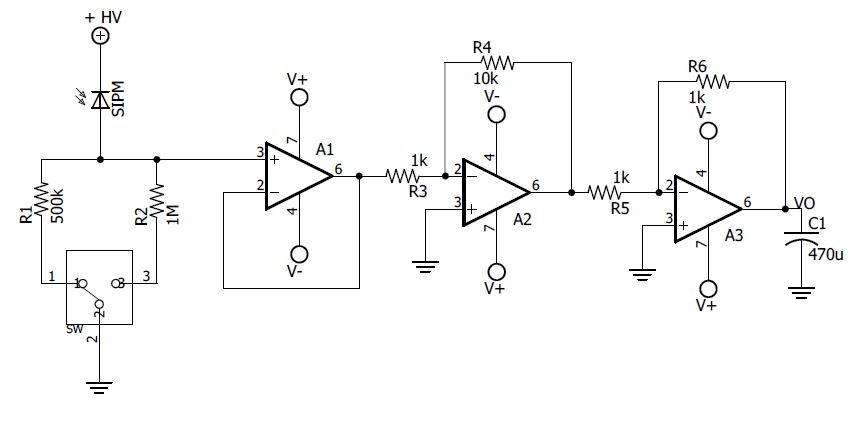
\includegraphics[width=0.8\textwidth]{Images/ammeter.JPG}
    \label{fig:ammeter}
  \par\end{centering}
\end{figure}
\\ \\
El circuito utilizado para implementar el medidor de corriente se muestra en la fig. \ref{fig:ammeter}, donde se pueden observar cuatro etapas. La primera etapa es la que realiza la conversión de corriente a voltaje por medio de $R_1$ o $R_2$, que pueden ser seleccionadas por medio del \textit{switch} SW en función de la magnitud de la corriente que genere el SiPM que esta polarizado por la fuente HV. \\ \\
La segunda etapa es un búfer que hace la adaptación de impedancias entre la primera etapa, que tiene una alta impedancia y la tercera etapa, que tiene una baja impedancia. La tercera etapa es un amplificador inversor con una ganancia de 10. Finalmente, la cuarta etapa es la etapa de salida y consiste en un filtro pasa bajas con una frecuencia de corte de $2.1$ Hz .\\ \\
El voltaje de salida $V_o$ es leído por una entrada analógica del microcontrolador Atmega 328, el cual tiene un ADC con una resolución de 10 bits y  puede mapear voltajes en el rango de 0 a 5 V, de forma que para definir los rangos de corriente se ajustaron los valores de $R_1, R_2, R_3, R_4, R_5~\mbox{y}~R_6$, teniendo dos rangos de medición de corriente en el instrumento ($2.5~\mbox{nA}$ a $500~\mbox{nA}$ y $2.5~\mbox{nA}$ $1~\mbox{uA}$) en función del valor de la resistencia de sensado utilizada ($1M\Omega~\mbox{o}~500~k\Omega$). Para estas configuraciones se tiene un \textit{Burden Voltage} máximo de $500~$mV.\\ \\
El amplificador operacional utilizado para $A_1, A_2~\mbox{y}~A_3$ es el OPA4228, sus principales características  son un \textit{Slew Rate} de $11 \mbox{V/}\mu\mbox{s}$, un ancho de banda de $33~$MHz, un voltaje \textit{Offset} de entrada de $\pm5~\mu$V, una corriente de polarización (Input Bias Current) de $\pm2.5$ nA, un rango del voltaje de alimentación de $\pm2.5$ V a $\pm18$~V.% y su valor comercial es de U\$ $5.48$.
\begin{table}[h!]
\caption{Principales parámetros eléctricos del amplificador operacional OPA4228.}
    \label{table_PID_c}
	\centering
	\begin{tabular}{ c  c  c}
    \hline
    Parámetro     & Típico     &   Máximo  \\ \hline
    \multicolumn{1}{c}{Input Offset Voltage}      & $\pm10~\mu$V        & $\pm200~\mu$V          \\
    \multicolumn{1}{c}{Input Bias Current}      & $\pm2.5$nA        & $\pm10$nA         \\ \hline
	\end{tabular}
\end{table}
\subsubsection{Análisis de Ruido del nanoamperímetro.}
Para el análisis de ruido se divide el circuito de medición de corriente en cada una de sus etapas, se identifican las fuentes de ruido y se calcula su contribución rms y pico-pico para el rango de frecuencia de interés ($0.1-2.1 $ Hz). El ruido dominante en este rango de frecuencias es el ruido flicker ($1/f$), por lo tanto para simplificar los cálculos se desprecia el ruido de banda ancha.
\begin{figure}[h!]
\begin{centering}

    \caption{Densidad espectral de ruido de entrada para corriente y voltaje del OPA4228. Adaptado de \citep{OPA_4228}. }
    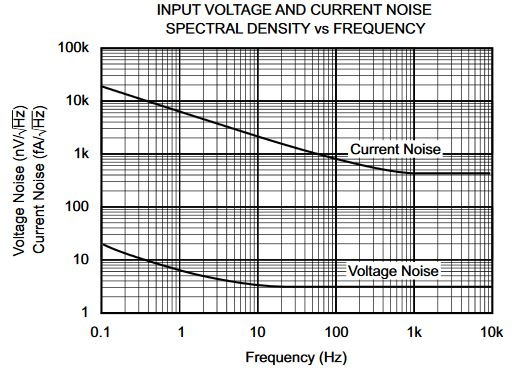
\includegraphics[width=0.6\textwidth]{Images/Noise_opa.JPG}
    \label{fig:noise_espectral}
  \par\end{centering}
\end{figure}
\begin{figure}[h!]
\begin{centering}
    \caption{Primera etapa del circuito de medición de corriente, compuesta por una resistencia de sensado y un búfer. }
    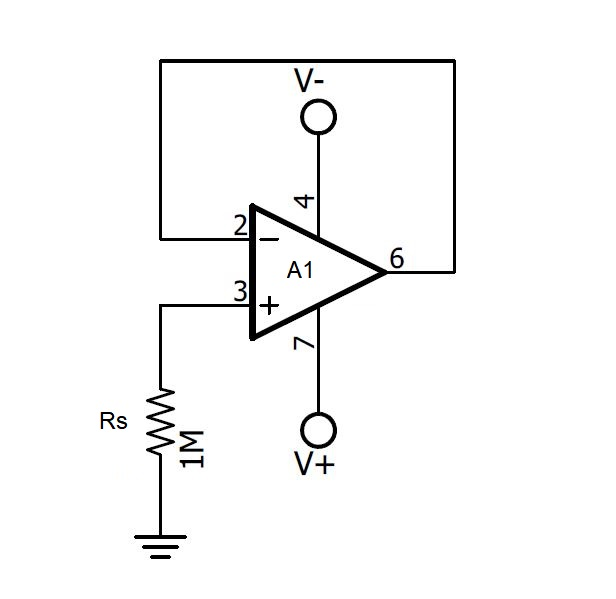
\includegraphics[width=0.35\textwidth]{Images/ammeter_buffer.JPG}
    \label{fig:ammeter_buffer}
  \par\end{centering}
\end{figure}
\\ \\
La primera etapa está compuesta por la resistencia de sensado y un búfer. Esta etapa es crítica en términos del ruido que aporta al circuito, debido al alto valor de la resistencia $R_s$ la cual posee ruido térmico y también convierte el ruido de corriente en ruido de voltaje. El ruido del amplificador para el rango de frecuencia de interés ($0.1-2.1 $ Hz) es $E_{nvflicker}$ y se calcula como: 
\begin{equation}
    E_{nNorm}=e_{nf}\sqrt{f_0}= 6.32~nV_{rms} ~,
    %E_{nNorm}=e_{nf}\sqrt{f_0}= \left (20~\mbox{nv}/\sqrt{Hz} \right)\sqrt{0.1\mbox{Hz}}= 6.32~nV_{rms}
    % E_{nNorm}&=& \left (20~\mbox{nv}/\sqrt{Hz} \right)\sqrt{0.1\mbox{Hz}}\\
    % E_{nNorm}&=& 6.32~nV_{rms}
\end{equation}
donde, $e_{nf}$ es la densidad espectral de ruido de voltaje  a la más baja frecuencia mostrada en la curva $1/f$, $f_{0}$ es la más baja frecuencia mostrada en la curva $1/f$ de la fig. \ref{fig:noise_espectral} y $E_{nNorm}$ es la densidad espectral de ruido normalizada a $1$ Hz, $f_H$ y $f_L$ son las frecuencias de corte superior e inferior de la curva $1/f$ respectivamente.\\  \\
\begin{equation}
    E_{nvflicker}=E_{nNorm}\sqrt{\ln\left(\frac{F_H}{F_L}\right)}=11.027~nV_{rms}.
    %E_{nvflicker}=E_{nNorm}\sqrt{\ln\left(\frac{F_H}{F_L}\right)}=6.32~nV_{rms}\sqrt{\ln\left(\frac{2.1}{0.1}\right)}=11.027~nV_{rms}
    % E_{nvflicker}&=&6.32~nV_{rms}\sqrt{\ln\left(\frac{2.1}{0.1}\right)}\\
    % E_{nvflicker}&=&11.027~nV_{rms}
\end{equation}
Otro componte de ruido es el ruido térmico y su densidad espectral de ruido  se calcula como:
\begin{equation}
    E_{nR}=\sqrt{4K_BTR_s\Delta f}= 181.98~nV_{rms},\\
    %E_{nR}&=& \sqrt{4K_BTR_s\Delta f}= \sqrt{4(1.38\times10^{-23}\mbox{J/K})(300\mbox{K})(1\times10^6\Omega)(2Hz)}\\%= 181.98~nV_{rms}\\
    % E_{nR}&=& \sqrt{4(1.38\times10^{-23}\mbox{J/K})(300\mbox{K})(1\times10^6\Omega)(2Hz)}\\
    % E_{nR}&=& 181.98~nV_{rms}
\end{equation}
donde, $K_B$ es la constante de \textit{Boltzmann}, $T$ es la temperatura absoluta en grados Kelvin, y $\Delta f$ es el ancho de banda para el que se calcula el ruido. El ruido de corriente tiene un efecto sobre el ruido de voltaje, este factor es:
\begin{equation}
    E_{niNorm}=(i_{nf}\times R_s)\sqrt{f_0}=6.32~\mu V_{rms}, \\
    %E_{niNorm}&=&(i_{nf}\times R_s)\sqrt{f_0}= \left (20~\mbox{pA}/\sqrt{Hz}\times10^6\Omega  \right)\sqrt{0.1\mbox{Hz}}\\
    %E_{niNorm}&=& \left (20~\mbox{pA}/\sqrt{Hz}\times10^6\Omega  \right)\sqrt{0.1\mbox{Hz}}\\
    %E_{niNorm}&=& 6.32~\mu V_{rms}
\end{equation}
donde, $E_{niNorm}$ es el ruido de voltaje causador por el ruido de corriente al pasar por $R_s$. 
\begin{equation}
    E_{niflicker}=E_{niNorm}\sqrt{\ln\left(\frac{F_H}{F_L}\right)}=11.035~\mu V_{rms}.\\
    %E_{niflicker}&=&E_{niNorm}\sqrt{\ln\left(\frac{F_H}{F_L}\right)}=6.32~\mu V_{rms}\sqrt{\ln\left(\frac{2.1}{0.1}\right)}\\
    %E_{niflicker}&=&6.32~\mu V_{rms}\sqrt{\ln\left(\frac{2.1}{0.1}\right)}\\
   % E_{niflicker}&=&11.035~\mu V_{rms}
\end{equation}
El ruido total es:
\begin{eqnarray}
    E_{nt}(rms)&=&\sqrt{(E_{nvflicker})^2+(E_{nR})^2+(E_{niflicker})^2};\\
    \label{ruido_total}
    %E_{nt}(rms)&=&\sqrt{(11.027\times10^{-9})^2+(181.98\times^{-9})^2+(11.04\times^{-6})^2}\\%= 11.036~\mu V_{rms}\\
     E_{nt}(rms)&=& 11.036~\mu V_{rms};\\
     E_{nt}(pp)&=& 6\times E_{nt}(rms)= 66.22~\mu V_{pp}.
     %E_{nt}(pp)&=& 66.22~\mu V_{pp}
\end{eqnarray}
Como se observa en la expresión \ref{ruido_total} el término $E_{niflicker}$ es dominante para valores muy grandes de $R_s$ \citep{noise_source}, por lo tanto los otros términos se pueden despreciar.\\ \\
Si se analizan las siguientes etapas del circuito de medición de corriente, la más crítica es la que tiene mayor ganancia (10). En esta etapa la resistencia equivalente que genera un ruido de voltaje referido  a la entrada es $R_3||R_4$ ($0.9~k\Omega$). De esta forma el ruido térmico es despreciable y el ruido de voltaje es el mismo que en la primer etapa  ($11,027~nV_{rms}$), igualmente despreciable. Asimismo, el ruido de voltaje relacionado con el paso del ruido de corriente por $R_3||R_4$ es despreciable comparado con el ruido de voltaje total en la primera etapa. Esto debido a el bajo valor de esta resistencia equivalente y la baja ganancia del ruido (101).\\\\
Por último, el ruido de voltaje referido a la salida del medidor de corriente es igual a el ruido en la primera etapa multiplicado por la ganancia de la segunda etapa.
\begin{equation}
     E_{ntOut}(pp)= 10\times E_{nt}=662.2~\mu V_{pp}.
      %E_{ntOut}(pp)&=&662.2~\mu V_{pp}
\end{equation}
Otro componente del error DC del circuito es el voltaje de \textit{offset} del amplificador. Teniendo en cuenta que el ADC utilizado cuenta con $10$ bits para un rango de 5 V la resolución es $4.88~$mV, el cual es mayor al ruido del voltaje del sistema y se puede considerar que el ruido no afectará considerablemente el circuito diseñado.\\ \\
Finalmente, en la figura \ref{fig:Inoise} se muestra el resultado de la medición de la corriente oscura en un SiPM antes de la región de avalancha. A partir de estas muestras, se calculó la desviación estándar $\sigma$ (0.24 nA) y el valor mínimo que se puede medir (2.12 nA)
% \begin{equation}
%     I_{pp} = 6\times \sigma= 1.44 nA
%     %I_{pp} &=& 1.44 nA
% \end{equation}
\begin{figure}[h!]
\begin{centering}
    \caption{Medición de la corriente oscura del SiPM, utilizada para calcular la desviación estándar de las muestras en la medición de corriente.}
    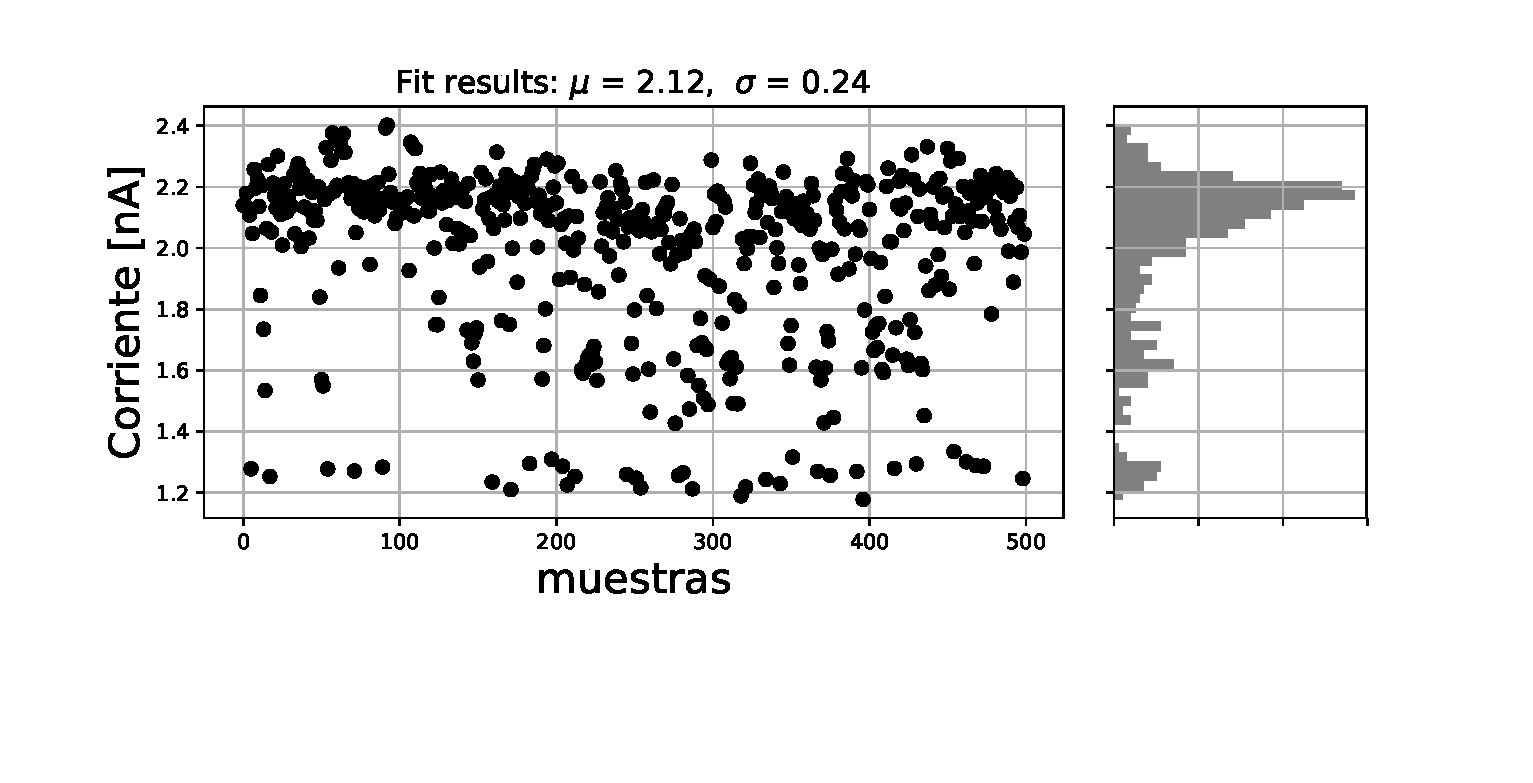
\includegraphics[width=\textwidth]{Images/Inoise.eps}
    \label{fig:Inoise}
  \par\end{centering}
\end{figure}
%%%%%%%%%%%%%%%%%%%%%%%%%%%%%%%%%%%%%%%%%%%%%%%%%%%%%%%%%%%%%%%%%%%%%%%%%%
\subsection{Fuente de polarización del SiPM.}
Un módulo indispensable para cualquiera de los procedimientos de caracterización es la fuente de polarización del SiPM. En este caso, se utilizó el módulo  C12332-01 de Hamamatsu, éste incluye una tarjeta con un sensor de temperatura (LM94021BIMGX de Texas Instruments)  y un soporte para ubicar el SiPM, adicionalmente cuenta con una fuente de voltaje C11204-01, una etapa de amplificación y una interfaz USB, como se muestra en la fig. \ref{fig:conexion_driverMPPC}.
\begin{table}[h!]
\caption{Características eléctricas del módulo  C12332-01 de Hamamatsu, utilizado para polarizar los SiPM.}
    \label{table_module_sorce}
	\centering
%    \begin{threeparttable}
	\begin{tabular}{ c  c  c}
    \hline
    Parámetro       & Valor típico   & Unidades     \\ \hline
    \multicolumn{1}{l}{Voltaje de alimentación}     & $\pm 5$        & V        \\
    \multicolumn{1}{l}{Rango de voltaje de salida}      & $40~\mbox{a}~80$        & V          \\
    \multicolumn{1}{l}{Consumo de corriente}      & $48$        & mA          \\
    \multicolumn{1}{l}{Resolución}      & $10$        & mV          \\
    \multicolumn{1}{l}{Frecuencia de corte del amplificador}      & $40$        & MHz          \\
    \multicolumn{1}{l}{Ganancia del amplificador}      & $92$        &     --      \\ \hline
	\end{tabular}	
%    \end{threeparttable}
\end{table}
\begin{figure}[h!]
\begin{centering}
    \caption{Ejemplo de conexión del módulo C12332-01 de Hamamatsu (\textit{power supply circuit board}). Adaptado de \citep{Driver_mppc}. La fuente de polarización del SiPM se alimenta con una fuente externa de $\pm$5 V  y su configuración se realiza por medio me una interfaz USB.}
   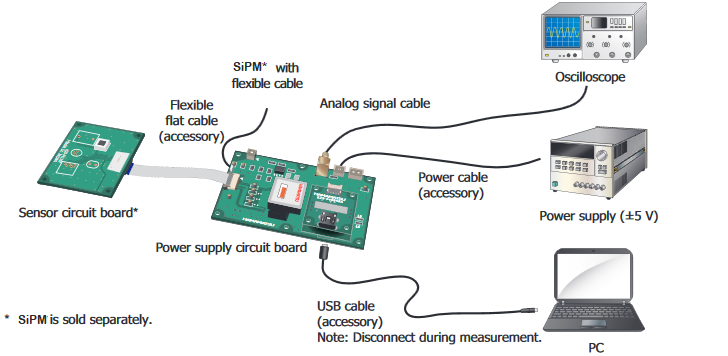
\includegraphics[width=0.8\textwidth]{Images/Source_module.PNG}
    \label{fig:conexion_driverMPPC}
  \par\end{centering}
\end{figure}
\\ \\
Asimismo, en la figura \ref{fig:interfase} se muestra la interfaz  gráfica del \textit{software} que controla el módulo. En el recuadro 1 se enciende o se apaga el módulo. En el recuadro 2, se puede ajustar el voltaje de operación y opcionalmente introducir los coeficientes de temperatura del SiPM  para realizar la compensación correspondiente. En el recuadro 3, se puede monitorear la temperatura, la corriente y el voltaje en el SiPM. Finalmente, en el recuadro 4, se muestra la conexión eléctrica típica del SiPM y la curva de dependencia del voltaje de operación en función de la temperatura. Este \textit{software} es compatible con un sistema operativo Microsoft\textsuperscript \textregistered$~$ Windows\textsuperscript \textregistered $~$7 (32-bits, 64-bits).

\begin{figure}[h!]
\begin{centering}
    \caption{Interfaz gráfica del \textit{software} que controla el módulo  C12332-01 de Hamamatsu, utilizado para polarizar los SiPM.}
    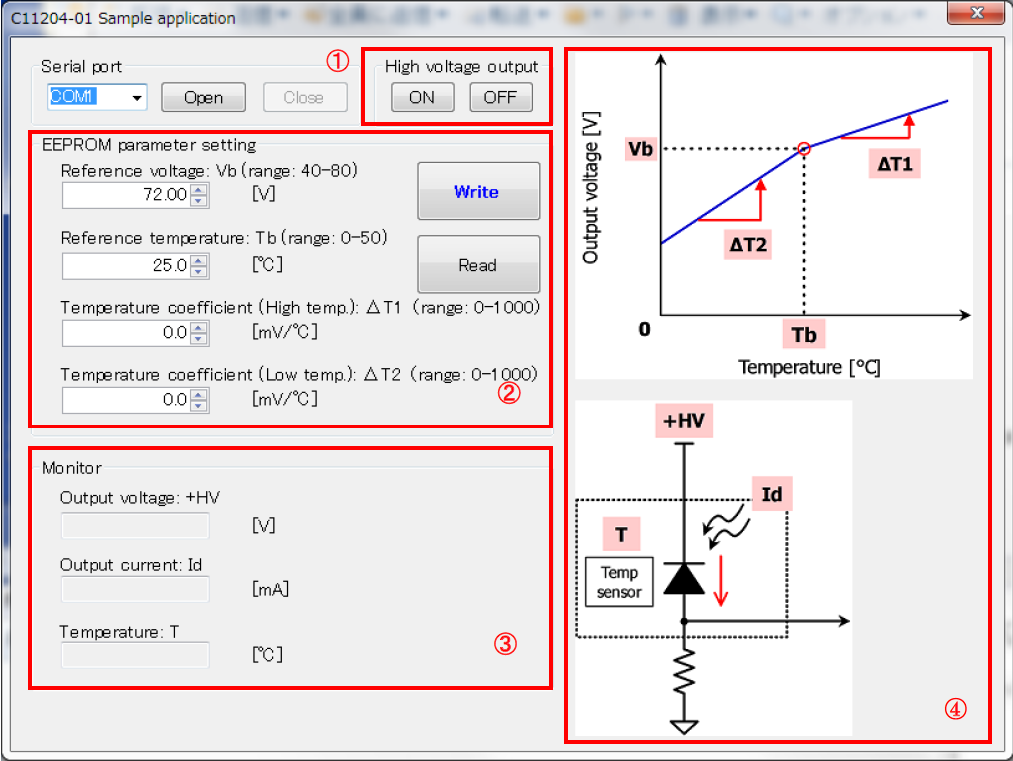
\includegraphics[width=0.7\textwidth]{Images/Source_Interfaz.PNG}
    \label{fig:interfase}
  \par\end{centering}
\end{figure}

%%%%%%%%%%%%%%%%%%%%%%%%%%%%%%%%%%%%%%%%%%%%%%%%%%%%%%%%%%%%%%%%%%%%%%%%%%
\section{MÓDULO DE CARACTERIZACIÓN DEL FOTÓN EQUIVALENTE Y LA GANANCIA.}
Para obtener el fotón equivalente (p.e.) y la ganancia del los SiPMs es necesario generar los histogramas de pico y de carga. Estos histogramas se pueden obtener mediante el análisis de los pulsos del SiPM cuando se realiza una estimulación controlada del dispositivo utilizando una fuente de luz pulsada.\\ \\
El histograma de pico representa gráficamente la frecuencia de ocurrencia de eventos con determinados valores máximos de voltaje, este histograma se caracteriza por tener picos que representan el número de fotones equivalentes, por consiguiente 1 p.e. está definido como la distancia entre dos picos consecutivos. Por otra parte, el histograma de carga se obtiene al realizar la integración numérica de los pulsos de corriente del SiPM, la diferencia entre los picos de este histograma es la carga en Coulombs de un pulso Geiger. Esta carga está directamente relacionada con la ganancia mediante la expresión \ref{Gain_eq}.       
\subsection{Fuente de luz pulsada.}
Para implementar una fuente de luz pulsada de baja intensidad es necesario crear una fuente de pulsos de voltaje que activen un LED de 470 nm. La fuente de luz pulsada es  empleada para estimular el SiPM de forma controlada en los experimentos que permiten obtener el valor de 1 p.e, la ganancia y la probabilidad de los tipos de ruido. Según \citep{Deisgn_LED_driver} el ancho de estos pulsos debe ser del orden de 10 ns, esto para emular el tiempo de respuesta de los pulsos de luz emitidos por los centelladores plásticos usados en los detectores de partículas.  
\begin{figure}[h!]
\begin{centering}
    \caption{Circuito utilizado para construcción de la fuente de luz pulsada, compuesto de dos etapas, una digital y otra analógica.}
    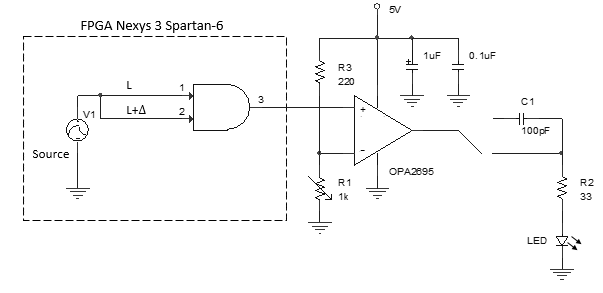
\includegraphics[width=0.7\textwidth]{Images/LED_circuit.PNG}
    \label{fig:LED_circuit}
  \par\end{centering}
\end{figure}
\\ \\
El circuito utilizado en la fuente de luz pulsada se presenta en la fig. \ref{fig:LED_circuit}. Inicialmente, se emplea una FPGA Nexys 3 Spartan-6 para generar dos pulsos periódicos con frecuencias entre 100 Hz y 25.6 kHz con un ancho de pulso de 30 ns, sincronizados con una señal de disparo (\textit{trigger})\footnote{https://github.com/juanvillafrades/Caracterizacion-SiPMs/tree/master/LEDPulser/PulseVariableGenerator}. Luego uno de estos pulsos se retarda usando una línea coaxial de 50 cm para posteriormente realizar una operación lógica (AND) entre éstos y generar un nuevo pulso con un ancho de 20 ns. Este nuevo pulso pasa por un amplificador en  modo comparador para reducir aún más el ancho mientras se aumenta su amplitud. \\ \\
El comparador utiliza un voltaje de referencia que se puede variar mediante el potenciómetro R1, para generar un pulso con un ancho de 6 ns a 11 ns y una amplitud entre 1.8 V y 3.7 V. Finalmente, mediante el capacitor C1 se puede eliminar la componente DC del pulso final.
%\begin{figure}[h!]
%    \caption{En azul el pulso que ingresa al comparador, en rojo el valor mínimo del pulso que estimula el LED.}
%    \label{fig:LED_Pulse_min}
%\begin{centering}
%  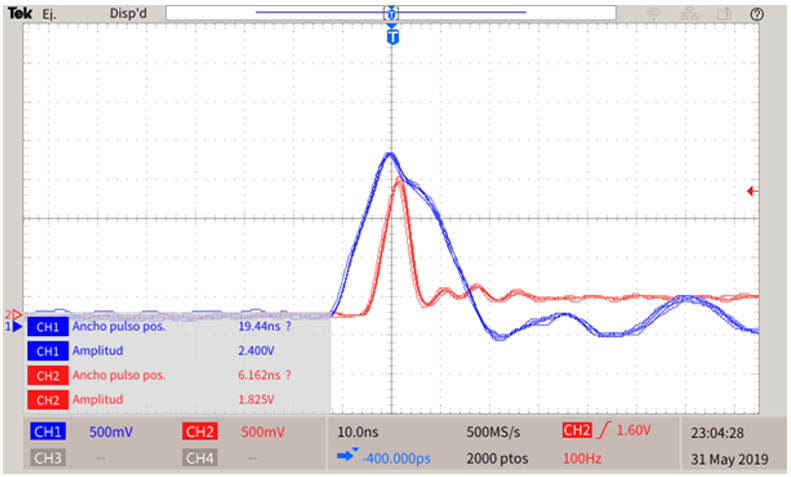
\includegraphics[scale=0.4]{Images/LED_Pulse_min.PNG}
%  \par\end{centering}
%\end{figure}
\begin{figure}[h!]
\begin{centering}
    \caption{Forma de los pulsos generados. En azul el pulso que ingresa al comparador, en rojo el pulso de salida con su máxima amplitud (3.7 V) sin componente DC. El FWHM (anchura a media altura) es menor a 10 ns.}
   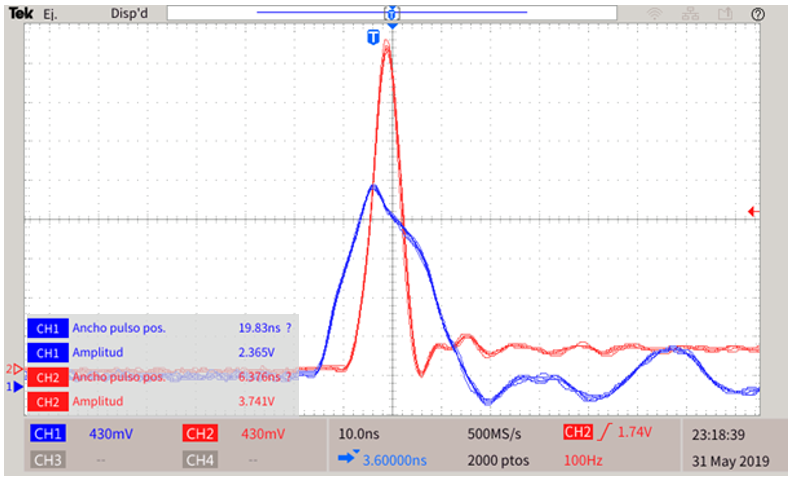
\includegraphics[width=0.7\textwidth]{Images/LED_Pulse_max.PNG}
    \label{fig:LED_Pulse_max}
  \par\end{centering}
\end{figure}
\\ \\
La técnica utilizada para el generador de pulsos se basa en \citep{Pulses_CFA}. Esta la idea consiste en usar un amplificador con realimentación de corriente como comparador. En este caso, el amplificador seleccionado es el OPA2695 de Texas Instruments, el criterio de selección fue el \textit{slew rate} y la corriente de salida que para este amplificador son $2900~\mbox{V}/\mu$s y 120 mA, respectivamente. Por otra parte, para generar los pulsos de luz se utilizó un LED azul difuso de 5 mm que emite fotones con una longitud de onda de 470 nm (longitud de onda de emisión típica en centelladores) y funciona con una corriente  de 30 mA. \\ \\
En la figura \ref{fig:LED_PCB} se muestra el circuito impreso en el que se implementó la fuente de luz pulsada, este módulo cuenta con un conector tipo MOD que le permite acoplarse a la FPGA. Así mismo, se utilizan conectores  SMA tipo hembra para los cables coaxiales RG59 de 50 Ohmios que llevan la señal de disparo y la señal que se retarda temporalmente, además se emplean conectores molex para el LED, el voltaje de polarización y el potenciómetro.
%\begin{figure}[h!]
%    \caption{}
%    \label{fig:LED_Pulse_max}
%\begin{centering}
%  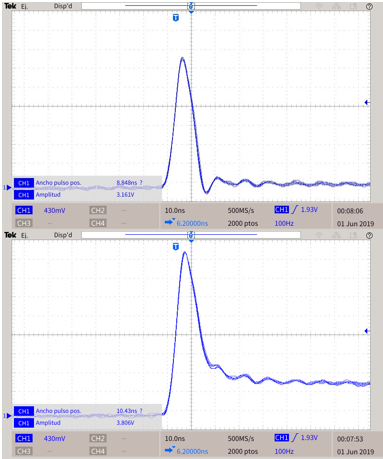
\includegraphics[scale=0.6]{Images/Pulse_cap_effect.PNG}
%  \par\end{centering}
%\end{figure}
\begin{figure}[h!]
\begin{centering}
    \caption{Circuito impreso con la implementación del amplificador comparador. Esta PCB se conecta a la FPGA para conformar la fuente de luz pulsada. }
    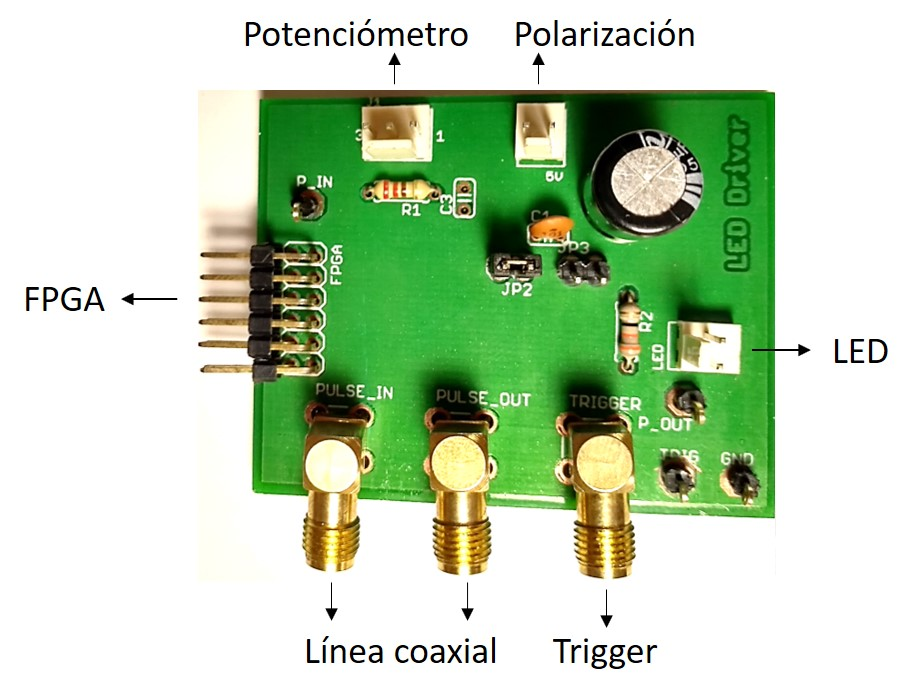
\includegraphics[width=0.5\textwidth]{Images/LED_PCB.jpg}
    \label{fig:LED_PCB}
  \par\end{centering}
\end{figure}
 %%%%%%%%%%%%%%%%%%%%%%%%%%%%%%%%%%%%%%%%%%%%%%%%%%%%%%%%%%%%%%%%%%%%%%%%%%
\subsection{Sistema de adquisición de datos.}
Para el registro y almacenamiento de los pulsos de los SiPM, en las pruebas en las que éstos se estimulan con la fuente de luz pulsada, se utiliza una Red Pitaya STEMlab 125-14. Esta es un tarjeta de desarrollo del tipo SBC (single-board computer) basada en un sistema operativo Linux, cuenta con una FPGA Xilinx Zynq 7010 SOC, un procesador Dual-Core ARM Cortex-A9 y una memora RAM de 4 Gb. Permite la adquisición, generación y procesamiento digital de señales de alta frecuencia. En la figura \ref{fig:Red_pitaya} se muestran sus principales características.   
\begin{figure}[h!]
\begin{centering}
    \caption{Red pitaya utilizada para la adquisición y almacenamiento de los  pulsos de los SiPM.}
    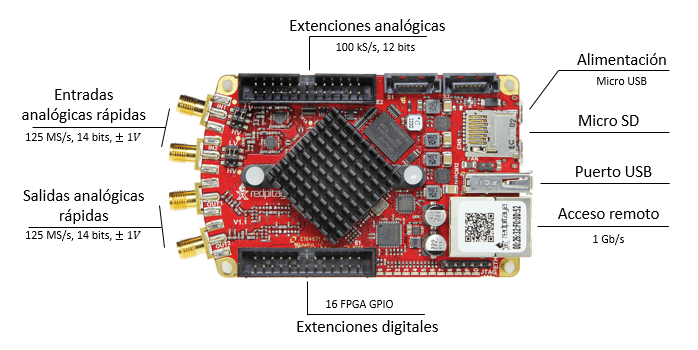
\includegraphics[width=0.8\textwidth]{Images/Red_pitaya.PNG}
    \label{fig:Red_pitaya}
  \par\end{centering}
\end{figure}
\\ \\
Los pulsos del SiPM son registrados con la Red Pitaya por medio de una de las entradas analógicas rápidas, con una frecuencia de muestreo de 125 MS/s y una resolución de 14 bits. Por otra parte, se utiliza una señal de disparo (trigger) para indicarle a la Red Pitaya cuándo debe realizar la digitalización de la entrada. La implementación del proceso de adquisición se realizó mediante un \textit{script} en Python \footnote{https://github.com/juanvillafrades/Caracterizacion-SiPMs/blob/master/Data\_Record.py} %%%% consultar como citar estoooooooooooooooooooooooooooooooooooooooooooooooo
desde el cual se puede configurar la frecuencia de muestreo, el número de eventos  que se desean registrar y la ventana temporal de adquisición en cada evento. Al finalizar la adquisición el \textit{script} genera un archivo de texto plano con todas las muestras de los pulsos registrados.\\ \\
La configuración experimental utilizada para el registro de datos se muestra en la fig. \ref{fig:Data_system}. Por otra parte, el acceso remoto a la red pitaya se realiza por medio de un protocolo SSH (Secure Shell) y el procesamiento y análisis de los datos adquiridos se realiza \textit{off-line}. 
\begin{figure}[h!]
\begin{centering}
    \caption{Diagrama del montaje utilizado para para registrar los eventos en el SiPM cuando este se estimula con la fuente de luz pulsada.}
    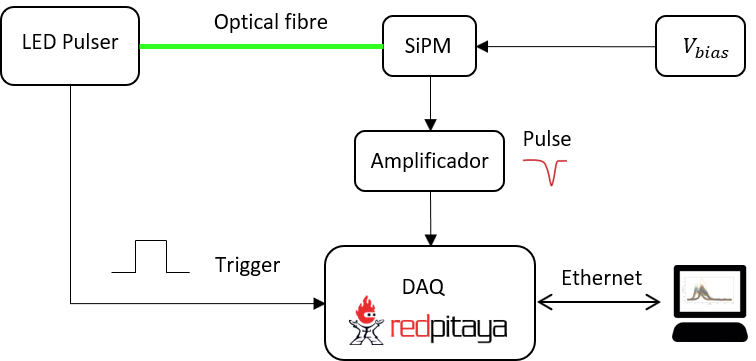
\includegraphics[width=0.6\textwidth]{Images/LED_diagrama.PNG}
    \label{fig:Data_system}
  \par\end{centering}
\end{figure}
%%%%%%%%%%%%%%%%%%%%%%%%%%%%%%%%%%%%%%%%%%%%%%%%%%%%%%%%%%%%%%%%%%%%%%%%%%
\section{RUIDO EN SIPMS}
Tanto el ruido correlacionado (\textit{crosstalk} y \textit{afterpulses}) como el no correlacionado (DCR) se obtienen del procesamiento de los datos registrados a partir de la configuración experimental mostrada en la fig. \ref{fig:Data_system}. El análisis de estos datos se realizó utilizando Python dentro del entorno de trabajo Jupyter\footnote{https://github.com/juanvillafrades/Caracterizacion-SiPMs/blob/master/Noise.ipynb}. Este procesamiento, consiste en primera medida, en un algoritmo que realiza un filtrado de los pulsos eliminando cualquier tipo de ruido debido a interferencias electromagnéticas, posteriormente se realiza una corrección de linea base (\textit{offset}) como se muestra en la fig. \ref{fig:PulsesNoise}.  
\begin{figure}[h!]
     \centering
        \caption{Pulsos de voltaje de un SiPM antes y después del preprocesamiento para filtrar ruido por interferencias electromagnéticas y eliminar el \textit{offset}.}
     \begin{subfigure}[b]{0.48\textwidth}
         \centering
         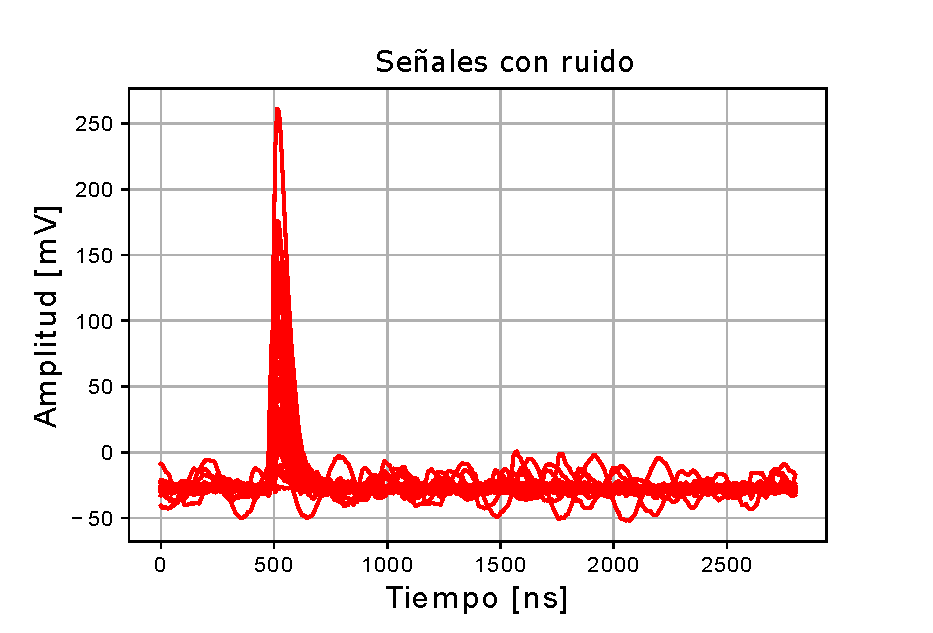
\includegraphics[width=\textwidth]{Images/Pulse_noise.eps}
         %\caption{}
         \label{fig:PulsesNoise1}
     \end{subfigure}
     %\hfill
     \begin{subfigure}[b]{0.48\textwidth}
         \centering
         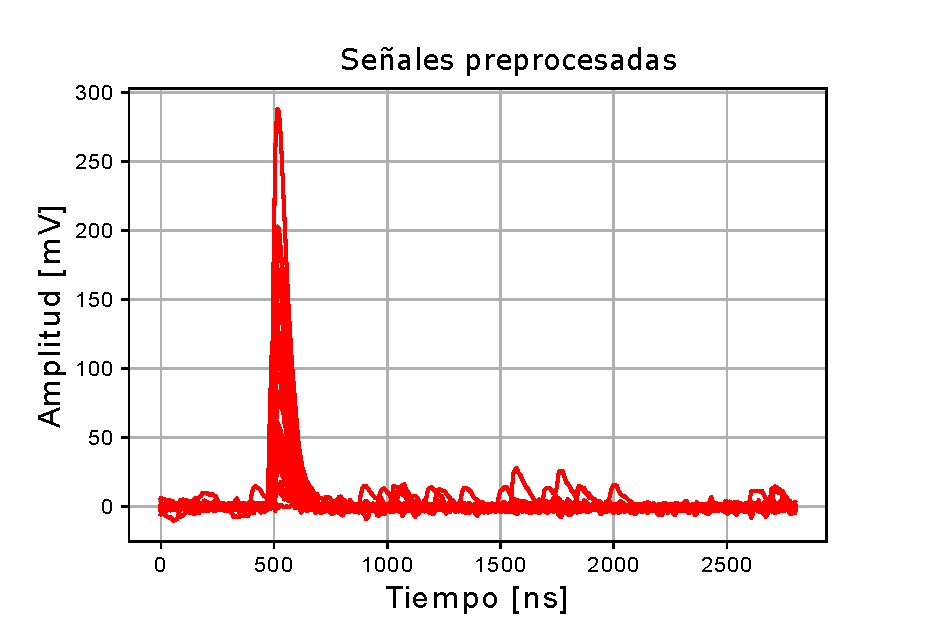
\includegraphics[width=\textwidth]{Images/Pulse_filter.eps}
         %\caption{}
         \label{fig:PulsesNoise2}
     \end{subfigure}
        \label{fig:PulsesNoise}
\end{figure}
\\ \\
Finalmente, se aplican los diferentes algoritmos que permiten realizar el cálculo de la probabilidad del ruido. El DCR se calcula como:
\begin{equation}
    DCR = \frac{N_{A1p.e.}}{W_{tA}N_p},
    \label{DCR_eq}
\end{equation}
donde, $N_{A1p.e.}$ es el número de eventos con una amplitud de 1 p.e. en una ventana de tiempo ($W_{tA}$) antes de los pulsos primarios y $N_p$ es el número total de eventos. Asimismo, la probabilidad de \textit{afterpulses} se calcula como:
\begin{equation}
    P_{AP} = \frac{N_{B1p.e.}-N_{A1p.e.}}{N_p}\times 100,\\
%    f_{AP} &=& \frac{N_{B1p.e.}}{W_{tB}N_p}-\frac{N_{A1p.e.}}{W_{tA}N_p}
    \label{AP_eq}
\end{equation}
donde, $N_{B1p.e}$ corresponde al número de eventos con una amplitud de 1 p.e. en una ventana de tiempo posterior a los pulsos primarios.
Por último, la probabilidad del \textit{crosstalk} se define como:
\begin{equation}
    P_{CT} =\frac{N_{2p.e.}}{N_p}\times 100,\\
%    f_{CT} &=& \frac{N_{2p.e.}}{W_{tB}N_p}
    \label{CT_eq}
\end{equation}
donde, $N_{2p.e.}$ significa el número de eventos con una amplitud de 2 p.e después de los pulsos primarios.\\ 
%%%%%%%%%%%%%%%%%%%%%%%%%%%%%%%%%%%%%%%%%%%%%%%%%%%%%%%%%%%%%%%%%%%%%%%%%%
